% ---------------------------------------------------------------------------------------------------------------
% TEMPLATE PARA TRABALHO DE MESTRADO
% Institudo Federal do Paraná - IFPR
% Customização da classe abnTeX2 (http://www.abntex.net.br/) para as normas da IFPR
%----------------------------------------------------------------------------------------------------------------
% Codificação: UTF-8
% LaTeX:  abnTeX2          
% ---------------------------------------------------------------------------------------------------------------


% CARREGA CLASSE PERSONALIZADA DA IFPR--------------------------------------------------------------------------
\documentclass[%twoside,                   % Impressão em frente e verso
    	        oneside,                   % Impressão apenas frentehttps://www.overleaf.com/project/601d9fdf130d22b45e6e96ff
]{configuracoes/utfpr-abntex2}


% INCLUI ARQUIVOS DE CONFIGURAÇÕES-------------------------------------------------------------------------------
% REFERÊNCIAS------------------------------------------------------------------
\usepackage[%
    alf,
    abnt-emphasize=bf,
    bibjustif,
    recuo=0cm,
    abnt-url-package=url,       % Utiliza o pacote url
    abnt-refinfo=yes,           % Utiliza o estilo bibliográfico abnt-refinfo
    abnt-etal-cite=3,
    abnt-etal-list=3,
    abnt-thesis-year=final
]{abntex2cite}                  % Configura as citações bibliográficas conforme a norma ABNT

% PACOTES----------------------------------------------------------------------
\usepackage[utf8]{inputenc}                                 % Codificação do documento
\usepackage[T1]{fontenc}                                    % Seleção de código de fonte
\usepackage{booktabs}                                       % Réguas horizontais em tabelas
\usepackage{color, colortbl}                                % Controle das cores
\usepackage{float}                                          % Necessário para tabelas/figuras em ambiente multi-colunas
\usepackage{graphics}
\usepackage{graphicx}% Inclusão de gráficos e figuras
\graphicspath{ {dados/figuras/} }
\usepackage{keystroke}
\usepackage{icomma}                                         % Uso de vírgulas em expressões matemáticas
\usepackage{indentfirst}                                    % Indenta o primeiro parágrafo de cada seção
\usepackage{microtype}                                      % Melhora a justificação do documento
\usepackage{multirow, array}                                % Permite tabelas com múltiplas linhas e colunas
\usepackage{subeqnarray}                                    % Permite subnumeração de equações
\usepackage{lastpage}                                       % Para encontrar última página do documento
\usepackage{verbatim}                                       % Permite apresentar texto tal como escrito no documento, ainda que sejam comandos Latex
\usepackage{amsfonts, amssymb, amsmath}                     % Fontes e símbolos matemáticos
\usepackage{amsmath}
\usepackage[algoruled, portuguese]{algorithm2e}             % Permite escrever algoritmos em português
%\usepackage[scaled]{helvet}                                % Usa a fonte Helvetica
\usepackage{times}                                          % Usa a fonte Times
%\usepackage{palatino}                                      % Usa a fonte Palatino
%\usepackage{lmodern}                                       % Usa a fonte Latin Modern
\usepackage[bottom]{footmisc}                               % Mantém as notas de rodapé sempre na mesma posição
\usepackage{ae, aecompl}                                    % Fontes de alta qualidade
\usepackage{latexsym}                                       % Símbolos matemáticos
\usepackage{lscape}                                         % Permite páginas em modo "paisagem"
%\usepackage{picinpar}                                      % Dispor imagens em parágrafos
%\usepackage{scalefnt}                                      % Permite redimensionar tamanho da fonte
%\usepackage{subfig}                                        % Posicionamento de figuras
%\usepackage{upgreek}                                       % Fonte letras gregas
\usepackage{tikz}											% Criar imagens vetoriais
\usepackage{microtype}
\usepackage{float}
\usepackage{ragged2e}
\usepackage{comment}
\usepackage{chemfig}
\usepackage{chemformula}
\usepackage{ccaption}
\usepackage{tocloft}

\newsubfloat{figure}

% Redefine a fonte para uma fonte similar a Arial (fonte Helvetica)
\renewcommand*\familydefault{\sfdefault}

%Novas defigições para teoremas
\newtheorem{definicao}{Definição}

%Novas simbolos
\newcommand{\gibbsm}{\underline{G}}
% CONFIGURAÇÕES DE APARÊNCIA DO PDF FINAL--------------------------------------
\makeatletter
\hypersetup{%
    portuguese,
    colorlinks=true,   % true: "links" coloridos; false: "links" em caixas de texto
    linkcolor=blue,    % Define cor dos "links" internos
    citecolor=blue,    % Define cor dos "links" para as referências bibliográficas
    filecolor=blue,    % Define cor dos "links" para arquivos
    urlcolor=blue,     % Define a cor dos "hiperlinks"
    breaklinks=true,
    pdftitle={\@title},
    pdfauthor={\@author},
    pdfkeywords={abnt, latex, abntex, abntex2}
}
\makeatother

% ALTERA O ASPECTO DA COR AZUL--------------------------------------------------
\definecolor{blue}{RGB}{0,0,0}

% REDEFINIÇÃO DE LABELS---------------------------------------------------------
\renewcommand{\algorithmautorefname}{Algoritmo}
\def\equationautorefname~#1\null{Equa\c c\~ao~(#1)\null}

% CRIA ÍNDICE REMISSIVO---------------------------------------------------------
\makeindex

% HIFENIZAÇÃO DE PALAVRAS QUE NÃO ESTÃO NO DICIONÁRIO---------------------------
\hyphenation{%
    qua-dros-cha-ve
    Kat-sa-gge-los
}



% INCLUI ARQUIVOS DO TRABALHO DE CONCLUSÃO DE CURSO (PRÉ-TEXTUAIS, TEXTUAIS, PÓS-TEXTUAIS)-----------------------

% INSERE CAPA E FOLHA DE ROSTO
% CAPA---------------------------------------------------------------------------------------------------

% ORIENTAÇÕES GERAIS-------------------------------------------------------------------------------------
% Caso algum dos campos não se aplique ao seu trabalho, como por exemplo,
% se não houve coorientador, apenas deixe vazio.
% Exemplos: 
% \coorientador{}
% \departamento{}

% DADOS DO TRABALHO--------------------------------------------------------------------------------------
\titulo{Aplicação do cálculo de equilíbrio de fase sólido-líquido para misturas binárias de diferentes compostos graxos e álcoois}
\titleabstract{}
\autor{Alex Issamu Moriya}
\autorcitacao{MORIYA, Alex Issamu} % Sobrenome em maiúsculo
\local{Umuarama}
\data{2021}

% NATUREZA DO TRABALHO-----------------------------------------------------------------------------------
% Opções: 
% - Trabalho de Conclusão de Curso (se for Graduação)
% - Dissertação (se for Mestrado)
% - Tese (se for Doutorado)
% - Projeto de Qualificação (se for Mestrado ou Doutorado)
\projeto{Dissertação}

% TÍTULO ACADÊMICO---------------------------------------------------------------------------------------
% Opções:
% - Bacharel ou Tecnólogo (Se a natureza for Trabalho de Conclusão de Curso)
% - Mestre (Se a natureza for Dissertação)
% - Doutor (Se a natureza for Tese)
% - Mestre ou Doutor (Se a natureza for Projeto de Qualificação)
\tituloAcademico{Mestre}

% ÁREA DE CONCENTRAÇÃO E LINHA DE PESQUISA---------------------------------------------------------------
% Se a natureza for Trabalho de Conclusão de Curso, deixe ambos os campos vazios
% Se for programa de Pós-graduação, indique a área de concentração e a linha de pesquisa
\areaconcentracao{}
\linhapesquisa{}

% DADOS DA INSTITUIÇÃO-----------------------------------------------------------------------------------
% Se a natureza for Trabalho de Conclusão de Curso, coloque o nome do curso de graduação em "programa"
% Formato para o logo da Instituição: \logoinstituicao{<escala>}{<caminho/nome do arquivo>}
\programa{PROGRAMA DE PÓS-GRADUAÇÃO EM SUSTENTABILIDADE}
\departamento{MESTRADO ACED\^{E}MICO ASSOCIADO}
\instituicaoS{Universidade Estadual de Maringá}
\instituicao{Instituto Federal do Paraná}
\logoinstituicao{0.15}{dados/figuras/Logo_PSU.jpg} 

% DADOS DOS ORIENTADORES---------------------------------------------------------------------------------
%\orientador{Nome do coorientador}
\orientador[Orientadora:]{Stella Alonso Rocha}
\instOrientador{IFPR}

%\coorientador{Nome do coorientador}
\coorientador[Coorientadora:]{Darliane Aparecida Martins}
\instCoorientador{IFPR}

% FOLHA DE ROSTO--------------------------------------------------------------------------------------------------------

% TRABALHO DE CONCLUSÃO DE CURSO
% \preambulo{{\imprimirprojeto} apresentado ao {\imprimirprograma} da {\imprimirinstituicao}, como requisito parcial para a obtenção do título de {\imprimirtituloAcademico}.}

% DISSERTAÇÃO DE MESTRADO
\preambulo{\large Dissertação de pesquisa apresentado no Conselho Acadêmico do Programa de Pós-Graduação em Sustentabilidade como parte integrante dos requisitos para a defesa de dissertação.}
%\preambulo{{\imprimirprojeto} apresentada ao Programa de \mbox{Pós-graduação} da {\imprimirinstituicao}, como requisito parcial para obtenção do título de {\imprimirtituloAcademico}.}

% TESE DE DOUTORADO
% \preambulo{{\imprimirprojeto} apresentada ao Programa de \mbox{Pós-graduação} da {\imprimirinstituicao}, como requisito parcial para a obtenção do título de {\imprimirtituloAcademico}.}

% PROJETO DE QUALIFICAÇÃO DE MESTRADO OU DOUTORADO
%\preambulo{{\imprimirprojeto} apresentado ao Programa de \mbox{Pós-graduação} da {\imprimirinstituicao}, como requisito parcial para a obtenção do título de {\imprimirtituloAcademico}.}

% OBSERVAÇÕES-----------------------------------------------------------------------------------------------------------
% Altere este arquivo APENAS comentando as linhas que não se aplicam ao tipo de trabalho acadêmico desejado.



\begin{document}

\pretextual
\imprimircapa                                               	           % Comando para imprimir Capa
\imprimirfolhaderosto{}                               		   % Comando para imprimir Folha de rosto
% INSERE ELEMENTOS PRÉ-TEXTUAIS
\begin{figure}[H]
   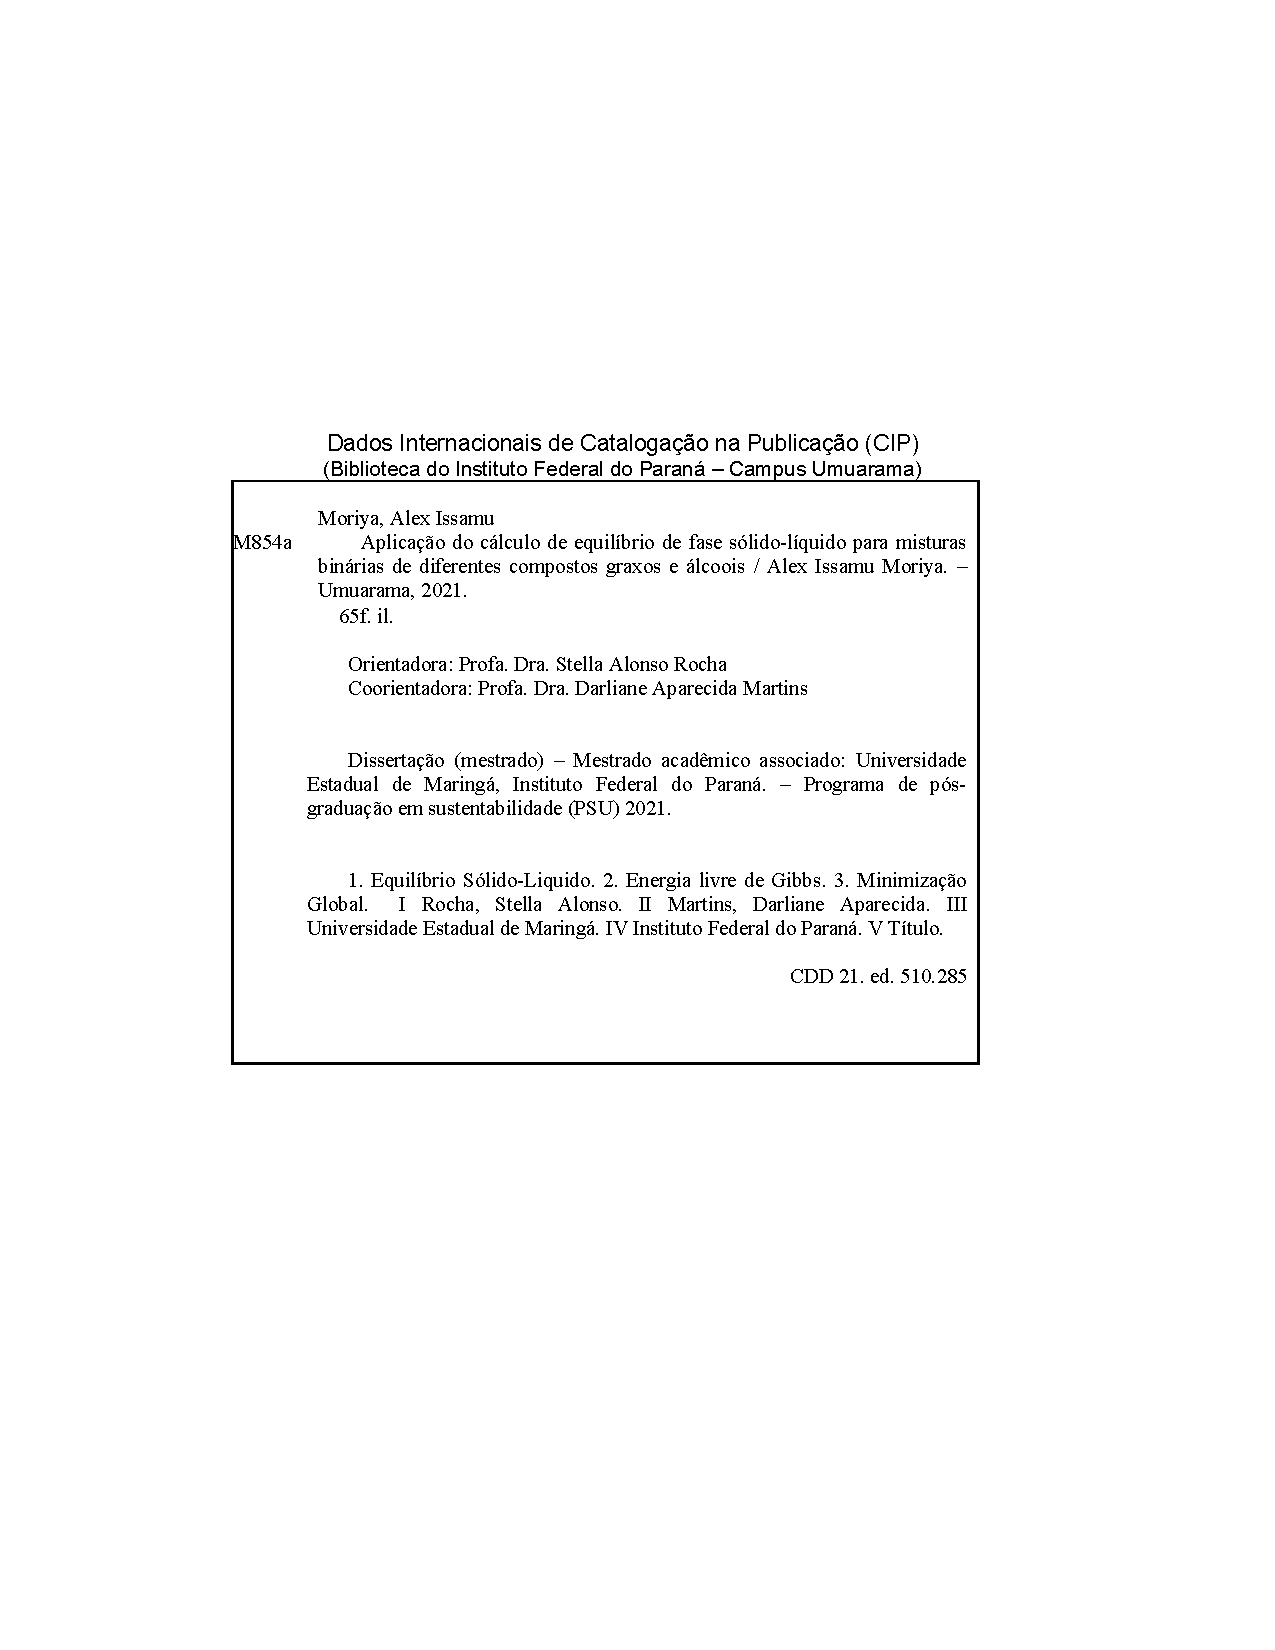
\includegraphics[width=1.1\linewidth]{dados/figuras/ficha catalografica Alex.pdf}
\end{figure}

\imprimirfolhadeaprovacao

% DEDICATÓRIA------------------------------------------------------------------

\renewcommand{\dedicatorianame}{DEDICATÓRIA}

\begin{dedicatoria}

Dedico esse trabalho ao meu pai Joaquim Toshiaki Moriya.

\end{dedicatoria}
          			   % Dedicatória
% AGRADECIMENTOS---------------------------------------------------------------

\begin{agradecimentos}[AGRADECIMENTOS]

Primeiramente agradeço a Deus, pela vida.

A minha esposa Vanessa Satiko Obana Haraki Moriya pela paciência e motivação ao meu filho por proporcionar alegria nestes momentos difíceis.

A orientadora Stella Alonso Rocha e coorientadora Darliane Aparecida Martins pela ajuda, paciência e contribuições para esse trabalho.

A Isaac Cirqueira Lopes e Otávio Akira Sakai a paciência, encaminhamentos dos documentos e tramites das burocracias.

Aos colegas de estudo que conheci ao decorrer dos estudos em particular, Edinei Aparecido Mora, Narliane de Melo Martins e Solano Ribeiro Soares.

\end{agradecimentos}
        			   % Agradecimentos
% EPÍGRAFE---------------------------------------------------------------------

\renewcommand{\epigraphname}{EPÍGRAFE}

\begin{epigrafe}

\textit{A matemática, olhada corretamente, possui não apenas verdade, mas suprema beleza, uma beleza fria e austera, como aquela da escultura, sem apelo a qualquer parte da nossa natureza mais fraca, sem as encantadoras armadilhas da pintura ou da música, mas sublimemente pura, e capaz de uma rigorosa perfeição que somente a maior das artes pode exibir. (RUSSELL, Bertrans, 1970).}

\end{epigrafe}

% OBSERVAÇÕES------------------------------------------------------------------
% Altere o texto para inserir a epígrafe do seu trabalho

              			   % Epígrafe
% RESUMO--------------------------------------------------------------------------------

\begin{resumo}[RESUMO]
\begin{SingleSpacing}


Os modelos termodinâmicos são utilizados com o intuito de determinar, de maneira satisfatória, o equilíbrio de fase sólido-líquido em diferentes soluções. Para este trabalho, os conceitos de modelagem matemática e otimização foram aplicados, com modelos termodinâmicos já definidos para misturas binárias de ácidos graxo e álcoois, com o propósito de obter a linha \textit{liquidus} e o(s) ponto eutético ou ponto peritético para os diagramas de fase estudados. Sendo assim, a característica deste trabalho é de desenvolvimento teórico, computacional, com foco na sustentabilidade, pela minimização na utilização de insumos e de resíduo ao meio ambiente; já que as análises dessas misturas de ácidos graxos e de álcoois foram todas realizadas com algoritmos computacionais, modelos termodinâmicos, modelagem matemática de Programação Não-Linear e teoria de equilíbrio de fases. Os softwares utilizados no trabalho foram: Gams, na implementação do algoritmo da programação não-linear com modelos termodinâmicos de Margules e Wilson com o solver CONOPT aplicado a análise dos dados de misturas binárias dos ácidos graxos e álcoois, para encontrar a minimização da energia livre de Gibbs do sistema; GEOGEBRA para coletar o dados de DSC (Calorimetria exploratória diferencial); PyCharm, junto com a biblioteca do R, na obtenção dos dados de temperatura e de mistura da planilha eletrônica para plotar os diagramas de fases e a linguagem \LaTeX como editor de texto, suas bibliotecas matemáticas e TIKZ. As misturas foram submetidas aos modelos termodinâmicos de Margules Simétrico, Margules Assimétrico e Wilson, configurados em equações explícitas em Temperatura ($T$), com intenção de obter o mínimo global a partir da minimização da Energia livre de Gibbs. Os sistemas estudados foram, Ácido Mirístico com Ácido Esteárico, Ácido Palmítico com Ácido Esteárico, Hexadecanol com Ácido Mirístico, Hexadecanol com Tetradecanol, Ácido Esteárico e Ácido Linoleico e Ácido Palmítico e Ácido Linoleico cujos diagramas de fases foram determinados e comparados graficamente com diagramas obtidos por técnicas calorimétricas disponíveis na literatura. Análises  quantitativas foram realizadas para a comprovação da proximidade entre os dados da modelagem e os dados experimentais citados. O estudo destes sistemas gerou informações sobre o comportamento de misturas de interesse das industrias de cosméticos, alimentos e combustíveis renováveis. Os modelos aplicados nesse trabalho sugerem que é possível aplicar as misturas de ácidos graxos e álcoois de origem vegetal nessas industrias contribuindo com o desenvolvimento sustentável. 

\vspace{1cm}

\textbf{Palavras-chave}:Equilíbrio Sólido-Liquido, Energia Livre de \textit{Gibbs}, Minimização Global.

\end{SingleSpacing}
\end{resumo}

% OBSERVAÇÕES---------------------------------------------------------------------------
% Altere o texto inserindo o Resumo do seu trabalho.
% Escolha de 3 a 5 palavras ou termos que descrevam bem o seu trabalho 

             			   % Resumo em Português
% ABSTRACT--------------------------------------------------------------------------------

\begin{resumo}[ABSTRACT]
\begin{SingleSpacing}


The thermodynamic models are used with the purpose of determining, in a satisfactory way, the balance of solid-liquid phase in different solutions. For this work, the concept of mathematical modeling and optimization were applied, with thermodynamic models already defined by binary mixtures of fatty acids and alcohols, in order to obtain the line liquidus and the eutectic point or peritectic point for the phase diagrams studied. Therefore, the characteristic of this work is of theoretical development, computational, with focus on sustainability, by the minimization in the use of input and of residue to the environment; since the analyses of these mixtures of fatty acids and alcohols were all accomplished with computational algorithms, thermodynamic models, mathematical modeling of Nonlinear Programming and phase balance theory. The softwares used in this work were: Gams, in the implementation of the algorithm of the nonlinear programming with thermodynamic models from Margules and Wilson with the solver CONOPT applied to the data analysis of the binary mixtures of fatty acids and alcohols, to find the minimization of the Gibbs free energy from the system; GEOGEBRA to collect the data of the articles of \textit{DSC} (Differential scanning calorimetry); \textit{PyCharm} together with the library of the \textit{R},  in the obtainment of the temperature data and of mixture of the electronic spreadsheet to plot the phases diagrams  and LATEX language as a text editor, its mathematical libraries and TIKZ. The mixtures were submitted to the thermodynamic models of Symmetrical Margules, Asymmetrical Margules and Wilson, configured in explicit equations in Temperature (T), in order to obtain the global minimum from the minimization of the Gibbs free energy. The systems studied were, Myristic Acid with Stearic Acid, Palmitic Acid with Stearic Acid, Hexadecanol with Myristic Acid, Hexadecanol with Tetradecanol, Stearic Acid and Linoleic Acid and Palmitic Acid and Linoleic Acid which phases diagrams were determined and graphically compared to diagrams obtained by available calorimetric techniques in the literature. Quantitative analyses were performed for the proof of proximity between the modeling data and the experimental data quoted. The study of these systems generated information about the behavior of the mixtures of the cosmetic industries interest, food and renewable fuels. The models applied in this work suggest that it is possible to apply the mixtures of fatty acids and alcohols of vegetable origin in these industries contributing to the sustainable development.
\vspace{1cm}
		
\textbf{Keywords}: Solid-Liquid Equilibrium, Free Gibbs Energy, Global Minimization.

\end{SingleSpacing}
\end{resumo}

% OBSERVAÇÕES---------------------------------------------------------------------------
% Altere o texto inserindo o Abstract do seu trabalho.
% Escolha de 3 a 5 palavras ou termos que descrevam bem o seu trabalho 
             		           % Resumo em Inglês
% Lista de Figuras----------------------------------------------------------------

\pdfbookmark[0]{\listfigurename}{lof}
\listoffigures*
\cleardoublepage

% OBSERVAÇÕES---------------------------------------------------------------------
% Este arquivo não precisa de ser alterado, pois a lista é gerada automaticamente.
   % Lista de Figuras
%% LISTA DE GRÁFICOS----------------------------------------------------------------

\renewcommand{\listofquadrosname}{LISTA DE GRÁFICOS}

\pdfbookmark[0]{\listofquadrosname}{loq}
\listofquadros*
\cleardoublepage

% OBSERVAÇÕES---------------------------------------------------------------------
% Este arquivo não necessita de ser editado. A lista é gerada automaticamente.
   % Lista de Quadros
% LISTA DE TABELAS-------------------------------------------------------------

\pdfbookmark[0]{\listtablename}{lot}
\listoftables*
\cleardoublepage

% OBSERVAÇÕES-------------------------------------------------------------------
% Este arquivo não precisa ser alterado, pois a lista é gerada automaticamente.
         		   % Lista de Tabelas
% LISTA DE ABREVIATURAS E SIGLAS----------------------------------------------------------

\begin{siglas}
    \item[DSC] Calorimetria exploratória diferencial
    \item[ESL] Equilíbrio sólido-líquido
    \item[GA] Algoritmo Genérico
    \item[GRG] Gradiente Reduzido Generalizado
    \item[NRTL] \textit{Nonrandom Two Liquid Theory}
    \item[PIM] Programação Inteira Mista linear
    \item[PL] Programação Linear
    \item[PNL] Programação Não-linear
    \item[UNIQUAC] \textit{Quasi-chemical Theory}
\end{siglas}

% OBSERVAÇÕES-----------------------------------------------------------------------------
% Altere a lista acima para definir os acrônimos e siglas utilizados neste trabalho
          		   % Lista de Abreviaturas e Siglas
% LISTA DE SÍMBOLOS------------------------------------------------------------

\begin{simbolos}
    \item[$R$] Constante universal dos gases
    \item[$\Delta H_{f}$] Entalpia de fusão
    \item[$f$] Fugacidade
    \item[$G$] Energia livre de Gibbs
    \item[$NC$] Número de componentes
    \item[$NF$] Número de fases
    \item[$A_{ij}$ ou $A_{12}$] Parâmetro de Margules
    \item[$\mu$] Potencial químico
    \item[$P$] Pressão
    \item[$T$] Temperatura
    \item[$T_{f}$] Temperatura de Fusão
    \item[$U$] Energia interna
    \item[$V$] Volume
    \item[$\underline{V}$] Volume molar
\end{simbolos}

% OBSERVAÇÕES-------------------------------------------------------------------
% Altere a lista acima para definir os símbolos utilizados no trabalho
        		   % Lista de Símbolos
%% LISTA DE ALGORITMOS----------------------------------------------------------

\newcommand{\algoritmoname}{Algoritmo}
\renewcommand{\listalgorithmcfname}{LISTA DE ALGORITMOS}

\floatname{algocf}{\algoritmoname}
\newlistof{listofalgoritmos}{loa}{\listalgoritmoname}
\newlistentry{algocf}{loa}{0}

\counterwithout{algocf}{chapter}
\renewcommand{\cftalgocfname}{\algoritmoname\space}
\renewcommand*{\cftalgocfaftersnum}{\hfill--\hfill}

\pdfbookmark[0]{\listalgorithmcfname}{loa}
\listofalgorithms
\cleardoublepage

% OBSERVAÇÕES------------------------------------------------------------------
% Este arquivo não precisa ser alterado, pois a lista é gerada automaticamente.
   % Lista de Algoritmos
% SUMÁRIO----------------------------------------------------------------------

\renewcommand{\contentsname}{SUMÁRIO}

\pdfbookmark[0]{\contentsname}{toc}
\tableofcontents*
\cleardoublepage

% OBSERVAÇÕES-------------------------------------------------------------------
% Este arquivo não precisa ser alterado, pois o sumário é gerado automaticamente.
               			   % Sumário

\textual
% INSERE ELEMENTOS TEXTUAIS
% INTRODUÇÃO-------------------------------------------------------------------

\chapter{INTRODUÇÃO}
\label{chap:introducao}

O estudo do equilíbrio de fases é de grande interesse nos processos químicos e em várias áreas. Informações sobre o equilíbrio sólido-líquido de misturas de ácidos graxos, ácido graxo e álcool, e álcoois são de interesse científico e industrial.  Nas indústrias de alimentos os procedimentos de emulsificação, aeração e técnicas de processamentos em alta pressão,  os quais tem como objetivo proporcionar várias texturas sem alterar o valor nutritivo, demandam por esses estudos. No setor do biodiesel, a determinação do \textit{cloud point} (ponto de nuvem ou ponto de turvação), indica a capacidade do biodiesel não solidificar durante seu uso como combustível. Na industria de cosmético está relacionado às emulsões. \cite{Leggieri2018a,Costa2007,Costa2009,Rocha2009a,Prausnitz,Rocha2011}

Prever quais fases e suas composições é  muito relevante em vários processos e operações da indústria. Essas fases podem ser  determinadas por meio de cálculos de equilíbrio de fase e análises de estabilidade. Os comportamentos do equilíbrio de fase para misturas sólido-líquido podem ser determinados, por calorimetria exploratória diferencial (DSC) ou por cálculos com modelos matemáticos. A aplicação de  modelos termodinâmicos químicos, como de  \textit{Wilson, Nonrandom Two Liquid Theory} (NRTL), Margules e \textit{Universal Quasi-chemical Theory (UNIQUAC)}, entre outros, tem o intuito de determinar os coeficientes de variedade. Dessa forma, os cálculos de equilíbrio de fase tem como objetivo, pela  minimização global da energia livre de \textit{Gibbs} com técnicas de otimização global, buscar e determinar pontos de transição da fase para a construção de seus respectivos diagramas para obtenção das linhas referentes a essas transições. \cite{Muller2019,Costa2009,Rocha2011,Farajnezhad2016}

 Portanto, esse trabalho propõe modelagens termodinâmicas para descrever o equilíbrio sólido-líquido de misturas binárias de ácidos carboxílicos e ou álcoois de  cadeias carbônicas longas, sendo então verificada a aplicação dos modelos de Margules, no formato Simétrico e Assimétrico, e Wilson. Uma melhor compreensão  desses equilíbrios  pode colaborar com o desenvolvimento  de  melhores  produtos,  princialmente,   o biodiesel que é uma alternativa, ambientalmente viável,  ao diesel.
%Introdução
%OBJETIVOS--------------------------------------------------------

\chapter{OBJETIVOS}
\label{chap:objetivos}

\section{Objetivo Geral}

O objetivo deste trabalho é utilizar modelos termodinâmicos capazes de indicar parâmetros para o equilíbrio de fase e determinar o diagrama de fase sólido-líquido por meio de modelagem matemática com recursos computacionais, com a finalidade de encontrar o \textit{Cloud Point}, ponto de turvação ou cristalização do biodiesel, além das outras aplicações industriais, com as misturas binárias encontradas na literatura com técnicas de DSC.

\section{Objetivo Específico}

Identificar quais os ácidos graxos e álcoois que são encontrados no biodiesel e quais são as proporções.

Buscar sistemas binários com métodos de DSC (Calorimetria exploratória diferencial) com misturas dos ácidos graxos e/ou álcoois, cuja a finalidade é implementar dos modelos termodinâmicos de Margules Assimétrico (MA), Margules Simétrico (MS) e Wilson.

Construir os diagramas de fase para cada método de DSC e comparar os valores encontrado com o Coeficiente de Determinação ou $R^2$.

Comparar os diagramas de fases dados experimentais via DSC com os calculados pelos modelos termodinâmicos.%Objetivos
% JUSTIFICATIVA------------------------------------------------------------------

\chapter{JUSTIFICATIVA}
\label{chap:justifiativa}

Um dos grandes interesses em compreender o equilíbrio de fase sólido-líquido para misturas graxas, é o estudo termodinâmico com a finalidade de estabelecer um modelo de cristalização para biodiesel, pois o biodiesel em baixas temperatura possui um ponto de turvação ou ponto de cristalização, chamado de \textit{Cloud Point}. Este ponto tem como característica a ocorrência da formação de cristais e como consequência, a menor fluidez do componente, o que não ocorre com combustível derivado do petróleo, inviabilizando sua comercialização.

Um dos pontos importantes é escolha das matérias-primas utilizadas na fabricação do biodiesel, as quais influenciam as propriedades do mesmo, segundo Dias (\citeyear{Angelica}), o óleo de Soja possui de 49,7\% até 56,9\% de Ácido Linoléico e de 9,9\% até 12,2\% de Ácido Palmítico em sua composição; o Óleo de Rícino possui de 2,9\% até 6,5\% de Ácido Linoléico e de 1,4\% até 2,1\% de Ácido Esteárico e o Óleo de Crambe possui 3,4\% de Ácido Palmítico e de 2,9\% até 6,5\% de Ácido Linoléico, dessa forma, diante diferenças de composições, estudar o comportamento das misturas binárias e seu comportamento termodinâmico tem sua relevância.

Ainda referente as composições, se a mistura possuir a fração elevada de  ácidos graxos insaturados, o combustível é mais vulnerável à oxidação;  tem pior capacidade de armazenamento,  menos fluidez no clima frio e menor estabilidade da oxidação. Estas características tornam mais difícil comercializar o biodiesel obtido de gorduras animais, que são mais insaturadas.  \cite{Leggieri2018a,Costa2012,Imahara2006}

%Os álcoois graxos,  que possuem entre 6 e 22 carbonos em sua cadeia, podem ser  extraídos  de plantas.  Essas molécula apresentam uma cadeia carbônica longa,  hidrofóbica,  e uma hidroxila, que permite que esses álcoois formem ligações de hidrogênio. Os álcoois graxos possuem variadas aplicações  industriais nos cosméticos suas aplicações  são como controladores de viscosidade, formadores de emulsões e emolientes; nos alimentos o uso desses álcoois resulta em diferentes texturas, nos fármacos desempenham um papel importante na temperatura de  fusão e solubilidade. \cite{Barbosa2012}

Aplicar modelos matemáticos a problemas reais pode auxiliar a tomada de decisão, contorna fases de teste diminuindo a formação de resíduos, padroniza a fabricação de produtos, além de ajudar na compreensão de fenômenos. As técnicas experimentais são vastamente utilizadas e confiáveis, como a técnica de Calorimetria Exploratória Diferencial (DSC), espectroscopia infravermelho com transformada de \textit{Fourier, Raman} ou difração de raio X; no entanto, utilizar modelos matemáticos tem suas vantagens, visto que, não necessita destes equipamentos e vai ao encontro dos princípios da química verde, que defende a utilização do mínimo de material logo minimiza os resíduos.\cite{DeMarco2019,Prausnitz,Goulart2019}

Um melhor entendimento sobre os equilíbrios sólido-líquidos das misturas graxas pode favorecer a produção de cosméticos, alimentos, fármacos e principalmente, biodiesel. \cite{Rocha2011,Leggieri2018a,Costa2007,Wei2009,Boudouh2016,Costa2012,Costa2009}

Esse trabalho utilizou de cálculos teóricos computacionais para o estudo do equilíbrio sólido-líquido de misturas de álcoois e ou ácidos graxos, permitindo um melhor entendimento do comportamento dessas misturas e sugere a possibilidade de utilização desses compostos, que podem ter origem vegetal em substituição a outros de origem fóssil.
%Justificativa
% REVISÃO BIBLIOGRÁFICA------------------------------------------------------------------

\chapter{REVISÃO DE LITERATURA}
\label{chap:revisao_bibliografica}
\section{Objetivos de desenvolvimento sustentável}

Os países membros da Organização das Nações Unidas (ONU), em 2015, estabeleceram uma agenda de desenvolvimento sustentável para os próximos 15 anos, na qual se comprometeram a trabalhar para atingirem 17 Objetivos de Desenvolvimento Sustentável (ODS).
“Os ODS buscam assegurar os direitos humanos, acabar com a pobreza, lutar contra a desigualdade e a injustiça, alcançar a igualdade de gênero e o empoderamento de mulheres e meninas, agir contra as mudanças climáticas, bem como enfrentar outros dos maiores desafios de nossos tempos” \cite{pactoglobal}.

Atualmente, petróleo bruto, carvão e gás, que são fosseis e não renováveis, ainda são dominantes na produção de combustíveis. A utilização dos combustíveis fosseis gera diversos impactos ambientais não desejáveis como: a poluição do ar e o aquecimento global \cite{Gebremariam2018}.

O petróleo, descoberto em 1859, foi a fonte de energia mais importante do  XX. Segundo  a Organização das Exportações de Petróleo Países, OPEP, a demanda mundial de óleo combustível atingirá até 109,4 milhões de barris por dia, em 2040, dos quais 5,7 milhões de barris por dia serão destinados a demanda de óleo diesel.

Dos 17 Objetivos de Desenvolvimento Sustentável três tem relação direta com a diminuição do consumo de combustíveis derivados de petróleo: o objetivo 7 - energia acessível e energia acessível e limpa; o objetivo 12 – consumo e produção responsáveis e o objetivo 13 – ação contra a mudança global do clima \cite{ONU}.

O biodiesel surge como uma das alternativas, ambientalmente vantajosas, que poderiam ser utilizadas para redução do consumo  dos combustíveis fosseis como fonte de energia . 

\section{Álcoois e Ácidos  carboxílicos}

Os ácidos carboxílicos com cadeia carbônica  entre 4 e 22 carbonos, e os  álcoois entre 6 e 22 carbonos, são denominados graxos. Ambos são encontrados em plantas, nas quais estão diretamente ligados.
    
Os álcoois graxos são, industrialmente, interessantes por terem a capacidade de formar micelas, são tensoativos não iônicos, ou seja, surfactantes. A indústria de cosméticos tem interesse por  moléculas que apresentam características hidrofóbicas e uma extremidade polar, o que permite a formação de emulsões. Outras aplicações possíveis são  a produção de lubrificantes,  polímeros, para o aumento de viscosidade em óleos,  em fragrância e flavorizantes. Nos alimentos eles possibilitam uma variedade de texturas. Nos  fármacos desempenha um papel importante nas propriedades  ponto de fusão e solubilidade, caracterizadas pelo equilíbrio de fase sólido-líquido. \cite{Barbosa2012}
    
Os ácidos graxos tem  aplicações nas indústrias de  biodiesel, de cosméticos, de alimentos, entre outras, dentre essas aplicações destaca-se  a fabricação de biodiesel. 

O biodiesel é um combustível  derivado de óleos vegetais, gorduras animais e óleos de algas. A substituição do diesel pelo biodiesel é ambientalmente benéfica, visto que, ele é biodegradável,  sua queima emite menos gases poluentes e  partículas \cite{Hanna1999,Atadashi2011}.   Para o biodiesel de origem vegetal  o CO$_2$  absorvido durante o crescimento da  planta,   é liberado durante a sua queima, estabelecendo um ciclo fechado de carbono. O uso do biodiesel reduz em até  78\% as emissões líquidas de CO$_2$ \cite{Aparecida2006}. 
    
O biodiesel é produzido por meio da transesterificação,  reação na qual  os triglicerídeos reagem com álcoois, na presença de um catalisador, para produzir esteres de  ácido graxo e glicerina, essa produzida como subproduto \cite{Hoekman2012}.
    
Ainda referente à produção, O  biodiesel pode ser produzido da maioria dos triglicerídeos, centenas de matérias-primas são descritas na literatura. No entanto, as mais  utilizadas são o óleo de soja nos Estados Unidos, óleo de colza na Europa, óleo de palma no sudeste Ásia e o Brasil, produz  variadas matérias-primas para a produção de biodiesel,  como a soja, o girassol, a mamona, o milho, o pinhão manso, o caroço de algodão, a canola, o babaçu, o buriti, o dendê, a macaúba e o amendoim, além das de origem animal como o sebo bovino e as gorduras de frango e de suínos, sendo o mais utilizado o biodiesel de soja \cite{Ramos2017,Hoekman2012}.
    
Os ácidos carboxílicos mais presentes nos biodieseis são mostrados na Tabela \ref{tab:Grupo} dieseis  derivados  de óleos vegetais e gorduras animais: ácido palmítico, ácido esteárico , ácido oleico, ácido linoléico e ácido linolênico. \cite{Hoekman2012,Ramos2017}.
    
\begin{table}[H]
    \centering
    \caption{Grupos de ácidos graxos típicos em biodiesel}
    \begin{tabular}{lccc}
    \hline
    Nome & N$^0$ CAS  & Fórmula Molecular  & Estrutura Molecular  \\
    \hline
    Ácido Láurico & 143-07-7 & \ch{C12H24O2} & \raisebox{-0.5\height}{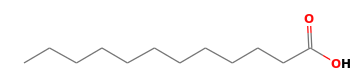
\includegraphics[width=0.4\linewidth]{dados/figuras/Ac_laurico.png}} \\
    Ácido Miristico & 544-63-8 & \ch{C14H28O2} & \raisebox{-0.5\height}{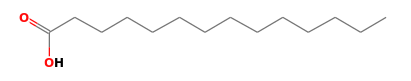
\includegraphics[width=0.4\linewidth]{dados/figuras/Ac_miristico.png}} \\
    Ácido Miristoléico & 544-63-9 & \ch{C14H28O2} & \raisebox{-0.5\height}{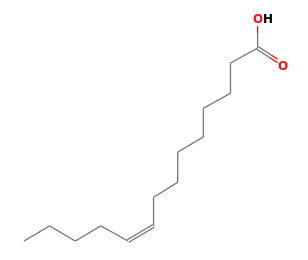
\includegraphics[width=0.25\linewidth]{dados/figuras/Ac_myristoleic.png}} \\
    Ácido Palmítico & 57-10-3 & \ch{C16H32O2} & \raisebox{-0.5\height}{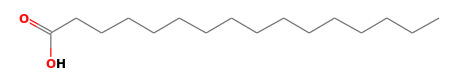
\includegraphics[width=0.4\linewidth]{dados/figuras/Ac_palmitico.png}} \\
    
    \end{tabular}
    \label{tab:Grupo}
\end{table}

\begin{table}[H]
    \centering
    \begin{tabular}{lccc}
    Ácido Palmitoléico & 373-49-9 & \ch{C16H32O2} & \raisebox{-0.5\height}{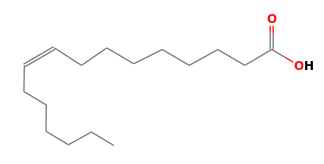
\includegraphics[width=0.3\linewidth]{dados/figuras/Ac_palmitoleico.png}} \\
    Ácido Esteárico & 57-11-4 & \ch{C18H36O2} & \raisebox{-0.5\height}{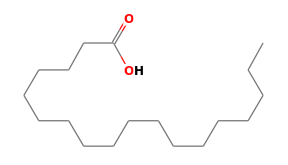
\includegraphics[width=0.4\linewidth]{dados/figuras/ac_estearico.png}} \\
    \end{tabular}
    \label{tab:2}
\end{table}
    
De acordo com o Ministério de Minas e Energia, atualmente,  o diesel de origem fóssil tem adição obrigatória de 13\% de biodiesel. Esse percentual deverá chegar a 15\% até 2023, como previsto na Resolução 16, de 2018, do Conselho Nacional de Política Energética (CNPE).
    
Esse consumo crescente de biodiesel leva a  necessidade de aumentar a produção do mesmo. A região  Noroeste do Paraná, localização de interesse deste trabalho, conta com 107 municípios, dentre eles,  Umuarama.  Os solos desta região, derivados do arenito, possuem elevado teor de areia e baixa porcentagem de argila, sendo extremamente friáveis e, consequentemente,  suscetíveis à erosão e ocorrência de deficiência de macro e micronutrientes \cite{Fonseca2005}.
    
A região  Noroeste do Paraná produz dentre outras culturas: \textit{Glycine max} (soja), \textit{Ricinus communis} (mamona) e \textit{Crambe abyssinica} (crambe), potenciais matérias-primas para o aumento da produção de biodiesel. A Tabela \ref{tab:angelica} observa-se a composição de ácidos graxos nesses óleos em percentagem \cite{Angelica}.

\begin{table}[H]
\centering
\caption{Composição dos ácidos graxos do óleo de soja, de rícino e de cambre.}
\begin{tabular}{lp{2.5cm}p{2.5cm}p{2.5cm}}
\hline
\multirow{2}{*}{Nomenclatura do Ácido} & \multicolumn{3}{l}{Porcentagem de ácidos carboxílicos totais (\%)}  \\
    & Soja  & Rícino & Crambe  \\
    \hline
     Ácido Láurico      & 0,1 (máx.)  &  & \\
     Ácido Mirístico    & 0,2 (máx.)  &  &  \\
     Ácido Palmítico    & 9,9 - 12,2  & 0,9 -1,5 & 3,4  \\
     Ácido Palmitoléico & Traços -0,2 &  &  \\
     Ácido Esteárico    & 3 - 5,4     & 1,4-2,1  & 1,1 \\
     Ácido Oleico       & 17,7 - 26   & 3,1-5,9 & 17,8 \\
     Ácido Linoléico    & 49,7 - 56,9 & 2,9- 6,5 & 6,1 \\
     Ácido Linolênico   & 5,5 - 9,5   &  & 2,8 \\
     Ácido Araquídico   & 0,2 - 0,5   &  & 1,7 \\
     Ácido Gadolêico    & 0,1 - 0,3   &  &  \\
     Ácido Behênico     & 0,3 - 0,7   &  & 3,7 \\
     Ácido Erúcico      & 0,3 (máx.)  &  & 56,7 \\
     Ácido Lignocérico  & 0,4 (máx.)  &  &  \\
     Ácido Eicosenóico  &             &  & 6,7 \\
     Ácido Ricinoléico  &             & 84,0 -91,0 &  \\
     \hline
\end{tabular}
\label{tab:angelica}
\end{table}

As propriedades, normalmente, avaliadas no biodiesel incluem viscosidade, número de cetano, ponto de nuvem, ponto de fluidez, ponto de entupimento do filtro frio, gravidade específica, ponto de inflamação, valor de iodo e valor de aquecimento. Várias dessas propriedades são influenciadas pelas estruturas ácidos graxos originais e do álcool utilizado \cite{Hoekman2012,Knothe2005}.

Uma das dificuldades à utilização do biodiesel é a formação de sólidos entupindo filtros e linhas de combustíveis que atrapalham o funcionamento e desempenho dos motores a diesel. Esse problema está diretamente relacionado aos pontos de fluidez (\textit{fluidity point}) e de ponto nuvem (\textit{cloud point}). O ponto de nuvem é a temperatura na qual o material graxo se torna nebuloso devido à formação de cristais e a solidificação e o ponto de fluidez é a temperatura mais baixa na qual ele ainda escoa \cite{Knothe2005}. 

Assim, para o desenvolvimento de melhores produtos, princialmente, biodieseis é importante compreender o equilíbrio de fases sólido-líquido das misturas de ácidos graxos e álcoois.

\section{Equilíbrio de fases sólido-líquido}
	
O estado termodinâmico de qualquer sistema multifásico depende de muitas variáveis, isto é, dadas as fases $\alpha$ e $\beta$ com vários componentes, o ponto de equilíbrio será obtido diante definição de uma temperatura $T$; das frações molares $x_{1}^{\alpha}, x_{2}^{\alpha}, \ldots$ e $x_{1}^{\beta}, x_{2}^{\beta}, \ldots$ das fases $\alpha$ e $\beta$ respectivamente e da pressão do sistema $P$ . Para que não ocorra ambiguidades o número de propriedades intensivas do estado de equilíbrio é definido pela \textit{regra de fases de Gibbs}. \cite{Prausnitz}
	
	%Número de propriedades intensivas = número de componentes - número de fases +2

	
Uma característica elementar na etapa I é definir de forma adequada e apropriada as funções matemáticas para evidenciar melhor a etapa II, graças a Gibbs, por definir o \textit{potencial químico}, a etapa II possui solução apropriada para o problema de equilíbrio de fases, indica-se o potencial químico por $\mu$, ou seja, potencial químico $\mu_{i}^{\alpha}$ se relaciona com $T$, $P$ e $x_{1}^{\alpha}, x_{2}^{\alpha}, \ldots$ e equivalentemente $\mu_{i}^{\beta}$ se relaciona com $T$, $P$ e $x_{1}^{\beta}, x_{2}^{\beta}, \ldots$. Para estabelecer essas relações, defini-se duas funções relacionadas ao potencial químico que são: a equação \textit{fugacidade} denotada por:
	
	\begin{equation}\label{eq:fugacidade1}
	\mu_{i}=\mu_{i}^{o}(T)+RT\ln\left(\dfrac{\widehat{f}_ {i}}{f_{io}}\right)
	\end{equation}
	em que $R$ é constante universal dos gases, $T$ é a temperatura, $\mu_{i}^{o}(T)$ potencial químico e $f$ a fugacidade. 
	E a outra, trata-se da ocorrência do equilíbrio sólido-líquido, em que $\alpha$ representa a fase sólida e $\beta$ a fase líquida, para obtenção da seguinte igualdade entre os potenciais químicos:
	\begin{equation}\label{eq:equilibrio1}
	\mu_{i}^{\alpha}=\mu_{i}^{\beta}
	\end{equation}
	analogamente para a fugacidade
	\begin{equation}
	\widehat{f}_ {i}^{\alpha}=\widehat{f}_ {i}^{\beta}
	\end{equation}
	
Uma outra maneira de representar o equilíbrio de fase quando $T$ e $P$ são constantes é pelo \textit{coeficiente de atividade}, cuja a definição é dada por:
	\begin{equation}\label{eq:coe_atividade}
	x_{i}^{L}\gamma_{i}^{L}f_{i}^{L}=x_{i}^{S}\gamma_{i}^{S}f_{i}^{S}
	\end{equation}
	em que é possível reescrevê-la da seguinte forma:
	\begin{equation}\label{eq:coe_atividade1}
	\dfrac{f_{i}^{L}}{f_{i}^{S}}=\dfrac{x_{i}^{S}\gamma_{i}^{S}}{x_{i}^{L}\gamma_{i}^{L}}
	\end{equation}
	em que $x_{i}^{L}$ é a fração molar da espécie $i$ na solução líquida e $x_{i}^{S}$ é a fração molar da espécie $i$ na solução sólida.
	\cite{SMITH2000,Rocha2009a,Prausnitz}
	
Obter critérios para misturas químicas e equilíbrio de fase, usa-se a notação indicadas por: $\eta_{ij}$, $\mu_{ij}$, $NC$ e $NF$ são respectivamente, o número de mol do componente $i$ na fase $j$, o potencial químico do componente $i$ na fase $j$, o número de componentes e o número de fases; envolvidas  nessas definições, o cálculo da \textit{energia de Gibbs} é definido por
	\begin{equation}\label{eq:minimo_globa_1}
	G=\sum_{i=1}^{NC}\sum_{j=1}^{NF}\mu_{ij} 
	\end{equation}
	em que, a partir da obtenção do mínimo global, denota-se a obtenção das condições necessárias e suficientes para o equilíbrio de fase.
	
Se o equilíbrio de fase for um sistema fechado, isto é,  $T$ e $P$ constantes, então o estado em que a energia de Gibbs alcança um valor mínimo, dentre os estados consistentes com a estequiometria da reação, resulta na identificação do estado de equilíbrio pela determinação da minimização da energia de Gibbs, sujeita as restrições estequiométricas conforme a equação (\ref{eq:minimo_globa_1}), isto é:
	\begin{description}
		\item[i)] número de mol deve ser um valor positivo:
		\begin{equation}
		\eta_{ij}\geqslant 0,\  \ i=1,2,\ldots,NC \mbox{ e } j=1,2,\ldots,NF
		\end{equation}
		\item[ii)] conservação de massa sem reações químicas:
		\begin{equation}
		\sum_{i=1}^{NC}\eta_{ij}=\eta_{i},\  \ i=1,2,\ldots,NC
		\end{equation}
	\end{description}
	em que $\eta_{i}$ é número total de mols do componente $i$.
	\cite{Sandlel,Barbosa2012,Prausnitz}
	
	\section{Cálculo do equilíbrio para substância pura}
	
	\hspace{5mm} O coeficiente de atividade para a fase líquida é definida para o estado padrão da substância líquida pura sub-resfriada na temperatura $T$ sobre uma pressão é representada pela equação:
	\begin{equation}\label{eq:atividade_1}x_i=\frac{f_{i(\mbox{\tiny sólido puro})}}{\gamma_{i}f_{i(\mbox{\tiny líquido sub-resfriado puro})}}
	\end{equation}
	para simplificar a notação
	\begin{equation*}
	f_{i}^{S}=f_{i(\mbox{\tiny sólido puro})}
	\end{equation*}
	e
	\begin{equation*}
	f_{i}^{L}=f_{i(\mbox{\tiny líquido sub-resfriado puro})}
	\end{equation*}
	em que as duas fugacidade depende apenas das propriedades da substância relacionada a componente $i$ e são independentes da natureza da substância. %A razão entre essas duas fugacidades.
	
A mudança de energia molar de Gibbs para o componente 2 está relacionada às fugacidades do sólido e do líquido sub-resfriado por como temperatura, concentração, pressão e natureza química das espécies. Assim para um sistema heterogêneo constituído de $NF$ número de fases e $NC$ número de componentes, a condição necessária para o equilíbrio de fase é descrita pela equação (\ref{eq:equi_fase_1}): \cite{Rocha2011,Sandlel,Barbosa2012,Prausnitz}:

\begin{equation}\label{eq:equi_fase_1}
	\begin{array}{ccccccc}
    	T^{1}&=&T^{2}&=&\cdots&=&T^{NF}\\
	P^{1}&=&P^{2}&=&\cdots&=&P^{NF}\\
	\mu_{1}^{1}&=&\mu_{1}^{2}&=&\cdots&=&\mu_{1}^{NF}\\
	\mu_{2}^{1}&=&\mu_{2}^{2}&=&\cdots&=&\mu_{2}^{NF}\\
	\vdots&=&\vdots&=&\cdots&=&\vdots\\
	\mu_{NC}^{1}&=&\mu_{NC}^{2}&=&\cdots&=&\mu_{NC}^{NF}\\
	\end{array} 
\end{equation}
em que $T$ é a temperatura, $P$ é a pressão e $\mu$ o potencial químico.

O equilíbrio de um sistema com $T$ e $P$ constantes é atingido quando a energia de Gibbs é mínima com relação ao número de mols, ocorre em uma determinada vizinhança do ponto quando se obtém a menor energia de Gibbs, descrita pela equação (\ref{eq:gibbs_1}):
	
\begin{equation}\label{eq:gibbs_1}
	(dG)_{T,P}\leq 0
\end{equation}

O equilíbrio estável está garantido quando o mínimo global da energia de Gibbs for encontrado \cite{Rocha2011}.

\section{Diagramas de fase - ESL}
	
Os diagramas de fases são a representação gráfica do comportamento da mistura binária dos compostos $A$ e $B$ em pressão constante, conforme Figura 2. O eixo das abscissas representa o percentual da mistura, o eixo das ordenadas indica a temperatura, as curvas mostram a transição de fase intitulada por \textit{linha liquidus}. Referente aos símbolos utilizados, $T_{f,B}$ representa a temperatura de fusão do componente $B$ puro e que a fração molar do componente $A$ é nula, isto é, $x_B=1$ e $x_A=0$ respectivamente, de modo análoga $T_{f,A}$ indica a temperatura de fusão do componente $A$ puro, $p$ e $e$ são os pontos \textit{peritéticos} e \textit{eutético} respectivamente. Acima da linha \textit{liquidus} identifica-se a fase líquida, sinalizada pela região com a letra L; a região entre a linha liquidus e os seguimentos de retas paralelas ao eixo das abscisas intersepta os pontos $p$ e $e$ são designadas por misturas de fases sólido$+$líquido, e a região abaixo dos seguimentos de reta são a fases sólida, representada na Figura \ref{fig:9}. \cite{Rocha2011}


\subsection{Pontos Eutético e Peritético}
	
\hspace{0.5cm} Ponto eutético ocorre quando uma mistura líquida durante o resfriamento atinge pelo menos duas fases sólidas. É o ponto no gráfico que mostra o equilíbrio delimita a transição de fase \cite{Rocha2011}. 

Ponto peritético é semelhante a eutética, ocorre em equilíbrio sólido-líquido de modo que uma fase sólida e outra fase líquida se transforma em outra fase distinta \cite{Rocha2011}.
	
Encontra-se os pontos eutético e peritético com a intersecção dos gráficos de pontos de invariância representados na Figura 3.


\section{Modelos termodinâmicos para descrição do equilíbrio de fase}
	
\subsection{UNIQUAC}
	
	O coeficiente de atividade $\gamma^{S}_{i}$ para a fase sólida, em que o modelo UNIQUAC é representado pelas (Eqs. \ref{eq:uniquac_1},\ref{eq:uniquac_2} e \ref{eq:uniquac_3}):
	
	\begin{equation}\label{eq:uniquac_1}
	\frac{g^{E}}{RT}=\sum_{i=1}^{n}x_{i} \ln\left(\frac{\Phi_{i}}{x_{i}}\right) + \frac{Z}{2}\sum_{i=1}^{n}q_{i} x_{i}\ln\left(\frac{\theta_{j}}{ \Phi_{i}}\right)-\sum_{i=1}^{n}x_{i} q_{i}\ln\left[\sum_{j=1}^{n}\theta_{j }\exp\left(\frac{\lambda_{ij}-\lambda_{jj}}{q_{i}RT}\right)\right]
	\end{equation}
	com
	\begin{equation}\label{eq:uniquac_2}
	\Phi_{i}=\frac{x_{i}r_{i}}{\displaystyle\sum_{j}x_{j}r_{j}}
	\end{equation}
	e
	\begin{equation}\label{eq:uniquac_3}
	\theta_{i}=\frac{x_{i}r_{i}}{\displaystyle\sum_{j}x_{j}r_{j}}
	\end{equation}
	os parâmetros estruturais $r$ e $q$ são dados pelas (Eqs. \ref{eq:parametro_1} e \ref{eq:parametro_2}) \cite{Coutinho2005,Coutinho2006}:
	\begin{equation}\label{eq:parametro_1}
	r_{i}=\frac{r_{iorg}}{6,744}=0,1C_{ni}+0,0672	
	\end{equation}
	\begin{equation}\label{eq:parametro_2}
	q_{i}=\frac{q_{iorg}}{5,4}=0,1C_{ni}+0,1141
	\end{equation}
	
Segundo ROCHA \citeyear{Rocha2011}, COSTA  \citeyear{Costa2007}, COUTINHO \citeyear{Coutinho2005} e COUTINHO \citeyear{Coutinho2006}, as equações \ref{eq:variacao_1} e \ref{eq:variacao_2} abaixo estimam a entalpia de substituição do cristal da molécula pura, da energia de interação entre duas moléculas idênticas, em que $Z$ é o número de correlação, $H$ é o átomo de hidrogênio e $\Upsilon$ é a variação:
	
	\begin{equation}\label{eq:variacao_1}
	\lambda_{ii}=-\frac{2}{Z}\left(\Upsilon_{sub}H_{i}-RT\right)
	\end{equation}
	
	E a energia de interação entre moléculas diferentes, em que $\alpha_{ij}$ indica pouco impacto na linha do diagrama
	
	\begin{equation}\label{eq:variacao_2}
	\lambda_{ij}=\lambda_{ji}=\lambda_{jj}(1-\alpha_{ij})
	\end{equation}
	
	\subsection{UNIFAC}
	
	A equação que representa o coeficiente de atividade UNIFAC , em que $\gamma_{i}^{C}$ termo condicional e $\gamma_{i}^{R}$ o termo residual, é dada pela (Eq. \ref{eq:coe_ativ_1}) \cite{Rocha2011}:
	
	\begin{equation}\label{eq:coe_ativ_1}
	\ln\gamma_{i}=\ln\gamma_{i}^{C}+\gamma_{i}^{R}
	\end{equation}
	
	Podendo escrever o termo combinatorial como mostra (Eqs. \ref{eq:combinatorial_1}, \ref{eq:combinatorial_2} e \ref{eq:combinatorial_3})
	
	\begin{equation}\label{eq:combinatorial_1}
	\ln\gamma_{i}^{C}=\ln\frac{\Phi_{i}}{x_{i}}+\frac{z}{2}q_{i}
	\end{equation}
	ou
	\begin{equation}\label{eq:combinatorial_2}
	\ln\gamma_{i}^{C}=\ln\frac{\Phi_{i}}{x_{i}}+\frac{z}{2}q_{i}\ln\frac{\theta_{i}}{\varphi_{i}}+l_{i}-\frac{\varphi_{i}}{x_{i}}\sum_{j}x_{j}l_{j}
	\end{equation}
	
	Onde
	
	\begin{equation}\label{eq:combinatorial_3}
	l_{i}=\frac{z}{2}(r_{i}-q_{i})-(r_{i}-1)
	\end{equation}
	
	\subsection{NRTL}
	
	A equação NRTL (Non Random Two Liquidis), em que as (Eqs. \ref{eq:nrtl_1}, \ref{eq:nrtl_2} e \ref{eq:nrtl_3}) representa pela energia de Gibbs em excesso, com $g_{ij}$ é o parâmetro de energia e $\alpha_{ij}$ é a não aleatoriedade da mistura:
	
	\begin{equation}\label{eq:nrtl_1}
	\ln\gamma_{i}=x_{i}^{2}\left[\tau_{ij} \left(\frac{G_{ij}}{x_{i}+x_{j}G_{ij}}\right)^{2}+\frac{\tau_{ij}G_{ij}}{(x_j+x_iG_{ij})^2}\right]
	\end{equation}
	onde
	\begin{equation}\label{eq:nrtl_2}
	\tau_{ij}=\frac{\Upsilon g_{ij}}{RT}
	\end{equation}
	e
	\begin{equation}\label{eq:nrtl_3}
	G_{ij}=\exp(-\alpha_{ij}\tau_{ij})
	\end{equation}
	
	\subsection{Margules}
	
	Equação de Margules (\ref{eq:Margules_2}), em que parâmetros de interação são indicados por $A_{ik}$, $A_{jk}$ e $A_{ij}$ e $x$ as fases molares:
	
\begin{equation}\label{eq:Margules_2}
	RT\ln\gamma_{k}=\frac{1}{2}\sum_{i=1}^{NC} \sum_{j=1}^{NC}(A_{ik}+A_{jk}-A_{ij})x_{i}x_{j}
\end{equation}
	
	\subsection{Wilson}
	
	A equação de Wilson (\ref{eq:Wilson_1}) indica a energia em excesso da mistura para um sistema binário com $n$ componentes e $n^{2}-n$ parâmetros ajustáveis \cite{Rocha2011}.
	\begin{equation}\label{eq:Wilson_1}
	\frac{G^{E}}{RT}=-\sum_{i}x_{i}\ln\left(1-\sum_{j}x_{j}\Lambda_{\frac{j}{i}}\right)
	\end{equation}
	em que $x_{i}$ é a fração molar e $\Lambda_{\frac{i}{j}}$ são parâmetros ajustáveis ($\Lambda_{ii}=0$, $\Lambda_{\frac{i}{j}}\neq\Lambda_{\frac{j}{i}}$). De maneira generalizada tem-se (Eqs. \ref{eq:Wilson_2}, \ref{eq:Wilson_3} e \ref{eq:Wilson_4}):
	\begin{equation}\label{eq:Wilson_2}
	\ln\gamma_{i}=1-\ln\sum_{j}x_{j}\Lambda_{ij}-\frac{\displaystyle\sum_{k}x_{k}\Lambda_{ki}} {\displaystyle\sum_{j}x_{j}\Lambda_{kj}}
	\end{equation}
	
	Os coeficientes de atividades ($\gamma$)
	\begin{equation}\label{eq:Wilson_3}
	\ln \gamma_{1}=-\ln(x_1+x_2\Lambda_{12} )+x_{2}\left(\frac{\Lambda_{12}}{x_1+x_2\Lambda_{12}}-\frac{\Lambda_{21}}{x_2+x_1\Lambda_{21}}\right)
	\end{equation}
	
	\begin{equation}\label{eq:Wilson_4}
	\ln \gamma_{2}=-\ln(x_2+x_1\Lambda_{21} )+x_{1}\left(\frac{\Lambda_{12}}{x_1+x_2\Lambda_{12}}-\frac{\Lambda_{21}}{x_2+x_1\Lambda_{21}}\right)
	\end{equation}
	
	\subsection{Slaugther e Doherty}
	
	\hspace{5mm} Para a determinação do diagrama de fase, será utilizada o modelo matemático do equilíbrio de fase sólido-líquido, segundo SLAUGHTER \& DOHERTY \citeyear{Douglas1995}, devemos considerar a condição de equilíbrio a igualdade do potencial quínico
	\begin{equation}\label{eq:slaugtther_1}
	\mu_{i}^{L}(T,P,x)=\mu_{i}^{S}(T,P,x)
	\end{equation}
	em que a equação \ref{eq:slaugtther_1} pode ser representada com uma combinação de componente puro do potencial químico da espécie $i$ em uma mistura:
	\\ Fase líquida
	\begin{equation}\label{eq:slaugtther_2}
	\mu_{i}^{L}(T,P,x)=\mu_{i}^{OL}+RT\ln(x_i\gamma_{i})
	\end{equation}
	Fase sólida 
	\begin{equation}\label{eq:slaugtther_3}
	\mu_{i}^{S}(T,P,x)=\mu_{i}^{OS}+RT\ln(x_i\gamma_{i}^{S})
	\end{equation}
	em que $\mu_{i}^{OL}$ e $\mu_{i}^{OS}$ são potenciais químicos para componentes puros. 
	Substituindo as equações \ref{eq:slaugtther_2} e \ref{eq:slaugtther_3} em \ref{eq:slaugtther_1}, adquirir-se
	\begin{equation}\label{eq:slaugtther_4}
	\mu_{i}^{OL}+RT\ln(x_i\gamma_{i}^{L})=\mu_{i}^{OS}+RT\ln(x_i\gamma_{i}^{S})
	\end{equation}
	ou
	\ref{eq:slaugtther_1}, provém
	\begin{equation}\label{eq:slaugtther_5}
	\dfrac{\mu_{i}^{OL}-\mu_{i}^{OS}}{RT}=\ln\dfrac{(x_i\gamma_{i}^{S}}{x_i\gamma_{i}}
	\end{equation}
	como manipulações matemáticas o modelo para o equilíbrio sólido-líquido (ESL) a equação usada é
	\begin{equation}\label{eq:slaugtther_6}
	x_i=\dfrac{z_i\gamma_{i}^{S}}{\gamma_{i}}\left\{\exp\left[\dfrac{\Delta h_{mi}^{O}}{R}\left(\dfrac{1}{T_ {mi}}-\dfrac{1}{T}\right)\right]\right\}
	\end{equation}
	onde de forma reduzida a equação \ref{eq:slaugtther_6}
	\begin{equation}\label{eq:slaugtther_7}
	x_i=\dfrac{1}{\gamma_{i}}\left\{\exp\left[\dfrac{\Delta h_{mi}^{O}}{R}\left(\dfrac{1}{T_ {mi}}-\dfrac{1}{T}\right)\right]\right\}
	\end{equation}
	Esta simplificação é usada em cálculos do diagrama de fases da curva sólida e líquida. 
	
	E para cálculos, a equação \ref{eq:slaugtther_7} do diagrama eutético para equilíbrio de massa é indicada por
	\begin{equation}\label{eq:slaugtther_8}
	\sum_{i_1}^{C}x_{i}=1
	\end{equation}
	e para o modelo do coeficiente de atividade usados em Wilson e Margules é indicada por
	\begin{equation}\label{eq:slaugtther_9}
	RT\ln\gamma_{k}=\dfrac{1}{2}\sum_{C}^{i=1}\sum_{C}^{j=1}(A_{ik}+A_{jk}-A_{ij})x_{i}x_{j}
	\end{equation}
	em que o processo de modificação do algoritmos das equações do equilíbrio de fases \ref{eq:slaugtther_7}, \ref{eq:slaugtther_8} e \ref{eq:slaugtther_9} são usadas para equilíbrio de fase vapor e líquido e aplica-se na fase sólida as equações:
	\begin{equation}\label{eq:slaugtther_10}
	K=\prod_{i=1}^{NC}(x_{i}^{S}\gamma_{i}^{S})^{vi}
	\end{equation}
	e
	\begin{equation}\label{eq:slaugtther_11}
	K=\exp\left(-\dfrac{\Delta G^O}{RT}\right)
	\end{equation}
	
	\section{Misturas de possíveis compostos para determinação equilíbrio sólido-líquido}
	
    O presente trabalho tem como parte dos objetivos determinar compostos de cadeia carbônica entre 10 e 20 carbonos com possíveis características para modelagem e identificação do ELS. Entre eles pode-se especificar cadeias lipídicas ou misturadas aos compostos álcoois. Entre elas, ácidos graxos saturados, insaturados, triacilgliceróis, esteres de etila, metila bisfenóis, entre outras possibilidades descritas nos subitens que seguem. Ainda, vale ressaltar que com a modelagem matemática proposta é possível determinar misturas binárias e também ternárias.
	
	Primeiramente, para iniciar a formulação e aplicar a modelagem em questão é necessário identificar os tipos de compostos a serem misturados, com a definição do ponto de fusão, a entalpia, estrutura e fórmula molecular desses compostos envolvidos \cite{Yaws2014a}.
	
	Os dados dos compostos como Entalpia $\Delta H_{f}$ e Ponto de Fusão $T_f$ foram pesquisados em YAWS \citeyear{Yaws2014}. A estrutura do composto, número do CAS (\textit{Chemical American Society}) ou registro CAS cuja a função é de registro único em um banco de dados do \textit{Chemical Abstracts Service}, uma divisão da \textit{Chemical American Society} e fórmula molecular foram obtidas nos dados do \textit{National Institute of Standards and Technology}. \citeyear{nist2020}
	
	\subsection{Ácido Mirístico}
	\label{sec:1}
	\begin{itemize}
		\item Estrutura
		\begin{figure}[H]
			\centering
			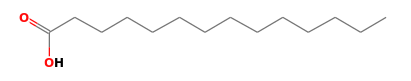
\includegraphics[width=0.7\linewidth]{dados/figuras/Ac_miristico.png}
			\caption[Ácido Mirístico]{Ácido Mirístico  NIST \textit{National Institute of Standards and Technology}}
			\label{fig:nist1}
		\end{figure}
		\item Número do CAS: 544-63-8
		\item Fórmula Molecular: \ch{C14H28O2}
		\item Temperatura de fusão ($T_f$)=327.55 k
		\item Entalpia ($\Delta H_{f}$)=10.771955 kcal/mol
	\end{itemize}
	
	\subsection{Ácido Esteárico}
	\label{sec:2}
	\begin{itemize}
		\item Estrutura
		\begin{figure}[H]
			\centering
			\includegraphics[width=0.7\linewidth]{dados/figuras/Ac_estearico.png}
			\caption[Ácido Esteárico]{Ácido Esteárico NIST \textit{National Institute of Standards and Technology}}
			\label{fig:nist2}
		\end{figure}
		\item Número do CAS: 57-11-4
		\item Fórmula Molecular: \ch{C18H36O2}
		\item Temperatura de fusão ($T_f$)=342.75 k
		\item Entalpia ($\Delta H_{f}$)=14.64126 kcal/mol
	\end{itemize}
	
	\subsection{Ácido Palmítico}
	\label{sec:3}
	\begin{itemize}
		\item Estrutura
		\begin{figure}[H]
			\centering
			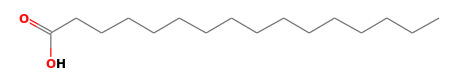
\includegraphics[width=0.65\linewidth]{dados/figuras/Ac_palmitico.png}
			\caption[Ácido Palmítico]{Ácido Palmítico NIST \textit{National Institute of Standards and Technology}}
			\label{fig:nist3}
		\end{figure}
		\item Número do CAS: 57-10-3
		\item Fórmula Molecular: \ch{C16H32O2}
		\item Temperatura de fusão ($T_f$)=336.00 k
		\item Entalpia ($\Delta H_{f}$)=80.252256 kcal/mol
	\end{itemize}
	
	\subsection{1-Hexadecanol}
	\label{sec:4}
	\begin{itemize}
		\item Estrutura
		\begin{figure}[H]
			\centering
			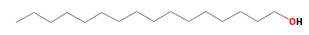
\includegraphics[width=0.8\linewidth]{dados/figuras/Hexadecanol.png}
			\caption[1-Hexadecanol]{1-Hexadecanol NIST \textit{National Institute of Standards and Technology}}
			\label{fig:8}
		\end{figure}
		\item Número do CAS: 36653-82-4
		\item Fórmula Molecular:\ch{C16H34O}
		\item Temperatura de fusão ($T_f$)=322,35k
		\item Entalpia ($\Delta H_{f}$)=8.025226 kcal/mol
	\end{itemize}
	


		%RevisãoBibliográfica
% MODELAGEM MATEMÁTICA PARA A OTIMIZAÇÃO DO EQUILÍBRIO SÓLIDO-LÍQUIDO------------------------------------------------------------------

\chapter{MODELAGEM MATEMÁTICA}
\label{chap:modelagem_matematica}

\section{Otimização}

O conceito de \textit{otimização} é uma forma de trazer uma solução satisfatória para problemas complexos que exigem a tomada de decisão ou alocação. Problema de decisão complexa, obtendo quantidade expressiva de valores correlacionadas com várias variáveis, foca-se em único objetivo projetado para quantificar o desempenho e medir a qualidade da decisão. Esse objetivo pode ser maximizado ou minimizado como as devidas restrições que pode limitar a seleção dos valores das variáveis de decisão e ajudar em sua escolha, como o objetivo de lucro ou perda em um ambiente de investimento ou de bem estar social. \cite{Luenberger2016}

\section{Programação Não Linear}

Problemas reais são na grande maioria formulados por restrições, como a política de produção em uma grande empresa ou planejamento da agência governamental, são problemas de programação não linear com restrições.

Em geral o problema de programação é indicada por:
\begin{equation}
\begin{array}{rcccc}
\mbox{minimização} & f(x) & & & \\
\mbox{sujeita as condições} & h_{i}(x)&=&a_{i}, & i=1,2,\ldots,m \\
& g_ {j}(x)&\leq&b_j, & j=1,2,\ldots,p\\
& x\in S & & & \\
\end{array}
\end{equation}

Em que $x$ é um vetor n-dimensional $x=(x_{1},x_{2},\ldots,x_{n})$, $f_{i}$ e $h_i$ são funções reais das variáveis $x_{1},x_{2},\ldots,x_{n}$. A função $f$ é a \textit{função objetivo}, $g$, $h$ e o conjunto $S$ são as restrições do problema; com os parâmetros $a_i$ e $b_j$. \cite{Luenberger2016, Rocha2009a}

\section{Convexidade}

Os conceitos relacionados aos conjuntos \textit{convexos} são relevantes teoria da otimização, representada pela Figura \ref{fig:convexSet} na forma bidimensional, que por sua vez é essencial para um estudante de otimização ter conhecimento de suas propriedades mais fundamentais. \cite{Luenberger2016, Rocha2009a}

\begin{definicao}
	Dado um conjunto $C\subset E^{n}$ diz que é \textbf{convexo} se para qualquer $x_{1}, x_{2} \in C$ e para todo $\alpha\in\mathbb{R}$, tal que o ponto $\alpha x_{1}+(1-\alpha)x_{2}\in C$.
\end{definicao}

%\begin{comment}
\begin{figure}[H]
	\centering
	\subbottom[Convexo]{
		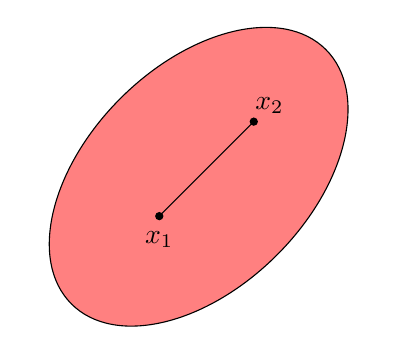
\begin{tikzpicture}
		\draw[rotate=-45,fill=red!50] (0,0) ellipse (40pt and 65pt);
		\draw (-0.5,-0.5) -- (0.7,0.7);
		\fill (-0.5,-0.5) circle[radius=1.5pt];
		\fill (0.7,0.7) circle[radius=1.5pt];
		\node at (-0.5,-0.8) {$x_1$};
		\node at (0.9,0.9) {$x_2$};
		\end{tikzpicture}}
	\hspace{2cm}
	\subbottom[Não Convexo]{
		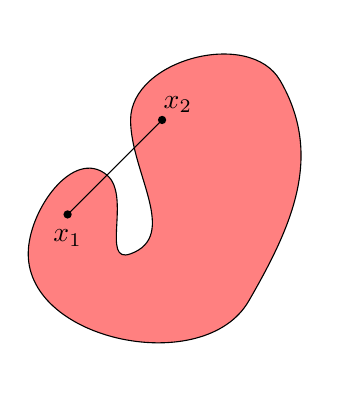
\begin{tikzpicture}
		\draw[fill=red!50] (0,0) to [out=140,in=90] (-1,-1)
		to [out=-90,in=240] (1.8,-1.6)
		to [out=60,in=-60] (2.2,1.2)
		to [out=120,in=90] (0.3,0.7)
		to [out=-90,in=20] (0.3,-1)
		to [out=200,in=-40] (0,0);
		\draw (-0.5,-0.5) -- (0.7,0.7);
		\fill (-0.5,-0.5) circle[radius=1.5pt];
		\fill (0.7,0.7) circle[radius=1.5pt];
		\node at (-0.5,-0.8) {$x_1$};
		\node at (0.9,0.9) {$x_2$};
		\end{tikzpicture}}
	\caption{Convexidade de conjuntos}
	\label{fig:convexSet}
\end{figure}

\section{\textit{Softwares} Utilizados}

Os \textit{softwares} utilizados para o desenvolvimento do trabalho, foram descritos nos subitens que seguem.

% TODO GEOGEBRA

\subsection{\textit{Geogebra}}
Para a coleta de pares ordenados e organização das misturas binárias para fins de cálculos vamos utilizar o \textit{software} \textit{Geogebra}\footnote{Site do Geogebra \url{https://www.geogebra.org/}} é um \textit{software} de código aberto Figura \ref{fig:11}, oferecido para várias plataformas, com a finalidade didática e de pesquisa. 
\begin{figure}[H]
	\centering
	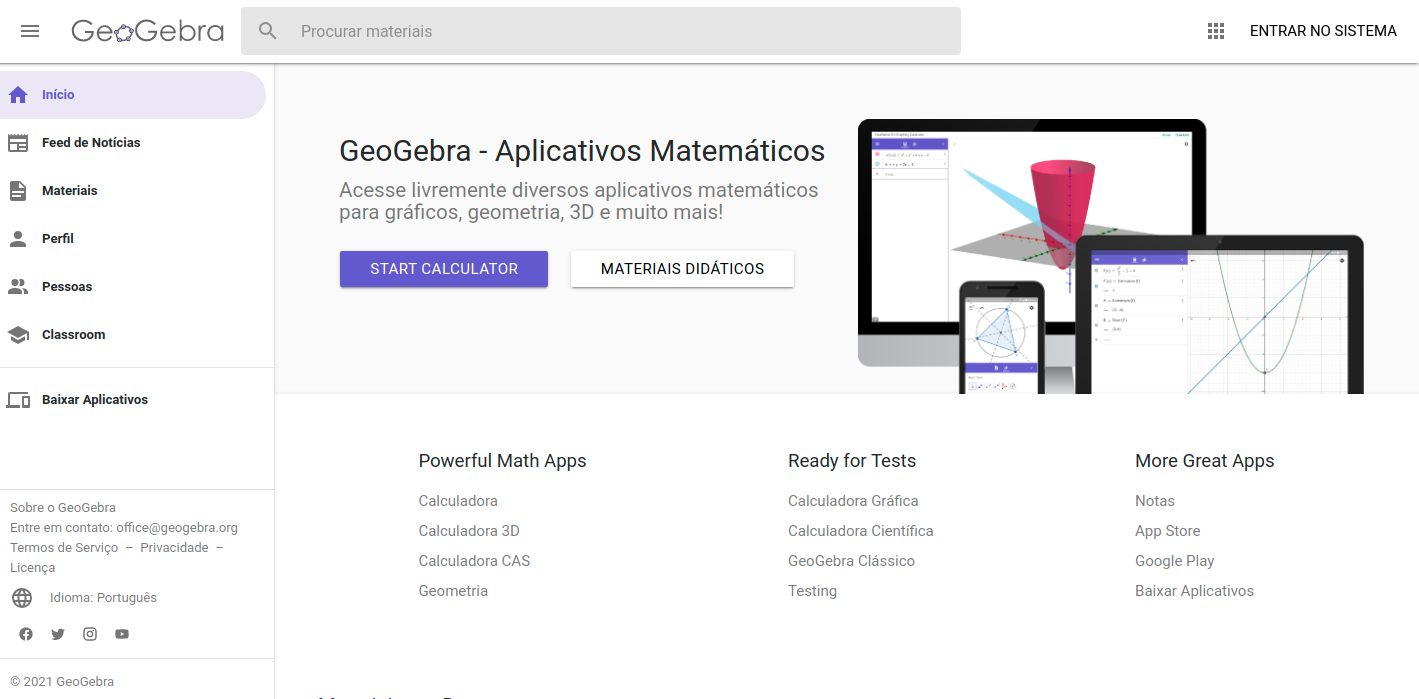
\includegraphics[width=0.9\linewidth 
	%,height=0.4\textheight
	]{dados/figuras/Geogebra_1.png}
	\caption[Site do Geogebra]{Site do Geogebra}
	\label{fig:11}
\end{figure}

\subsection{\textit{GAMS} General Algebric Model System}

O \textit{software} \textit{GAMS}\footnote{Site do GAMS \url{https://www.gams.com/}} é uma sistema de modelagem algébrica, desenvolvido para determinar soluções de sistemas com algoritmos matemáticos e otimização Figura \ref{fig:14}. O \textit{software} \textit{GAMS} com \textit{solver} comercial, para resolver modelos com aplicações em grande escala, com pacotes de testes \textit{GAMS} fornece modelos algébrico em código C, Delphi, Java e Fortran. 

\begin{figure}[H]
	\centering
	\includegraphics[width=1.0\linewidth 
	%,height=0.4\textheight
	]{dados/figuras/Gams_1.png}
	\caption[Site do \textit{GAMS}]{Site do \textit{GAMS}}
	\label{fig:14}
\end{figure}

\subsection{\textit{PyCharm} e \textit{R}}

Os \textit{software} \textit{PyCharm}\footnote{Site do \textit{PyCharm} \url{https://www.jetbrains.com/pt-br/pycharm/}} (FIGURA \ref{fig:15}) possui licença gratuita com restrições, disponíveis para as principais plataformas e, conjuntamente com a utilização da biblioteca \textit{R}\footnote{A base de dados para implementação de modelos estatísticos disponível no site \url{https://cran.r-project.org/}} (FIGURA \ref{fig:16}), se apresentam como uma base para implementação de algoritmos e modelos estatísticos. 

O \textit{PyCharm} possui uma IDE (Ambiente de Desenvolvimento Integrado) completa e simples para realizar o trabalho. A integração das bibliotecas ou  \textit{plugins} do \textit{software} traz melhor experiência, possui muitos tutoriais para melhor encaminhamento. Para esse trabalho, este \textit{software} foi usado na construção dos diagramas de fases junto com o \textit{R} para uma melhor perspectiva e pela facilidade de montar os algoritmos para tal aplicação. A biblioteca do \textit{R} auxiliou nos cálculos da Soma de Quadrado de Erro e no Coeficiente de Determinação forma dinâmica, contribuindo na escolha do modelo estatístico na comparação da técnica de DSC (Calorimetria Exploratória Diferencial) com os modelos termodinâmicos de Margules Simétrico, Margules Assimétrico e Wilson.
\begin{figure}[H]
	\centering
	\includegraphics[width=1.0\linewidth 
	%,height=0.4\textheight
	]{dados/figuras/Pycharm_1.png}
	\caption[Site do \textit{PyCharm}]{Site do \textit{PyCharm}}
	\label{fig:15}
\end{figure}
\begin{figure}[H]
	\centering
	\includegraphics[width=1.0\linewidth 
	%,height=0.4\textheight
	]{dados/figuras/R_1.png}
	\caption[Site do projeto R]{Site do projeto R}
	\label{fig:16}
\end{figure}

\subsection{Editor de texto \LaTeXe}

\LaTeXe  é o \textit{software} de código aberto de alta qualidade afim de produzir impressões profissionais e arquivos PDF, cuja base de dados \textit{TexLive}\footnote{Se encontra no site \url{http://tug.org/texlive/}} para plataformas Linux e macOS, organizada por \textit{TeX User Group} instituição sem fins lucrativos fundada em 1980, composto por \TeX\ \ criado por Donald Knuth e a mais conhecida ou difundida \textit{MikTex}\footnote{Se encontra no site \url{https://miktex.org/}} para todas as plataforma. A interface gráfica foi utilizado o \textit{TeXstudio}\footnote{Se encontra no site \url{https://www.texstudio.org/}} e \textit{Overleaf}\footnote{Se encontra no site \url{https://pt.sharelatex.com/}} uma ferramenta online para trabalhos colaborativos com o sistema de versionamento podendo ver quais são as modificações feitas por cada um colaborador. A a principal finalidade do \LaTeX é trazer uma tipografia de alta qualidade com o intuito trazer uma leitura mais agradável visualmente, com a biblioteca \textit{amsmath} para escrever fórmulas matemática, \textit{tikz} para criar desenhos vetoriais como os desenhos Figura\ref{fig:convexSet} e Figura\ref{fig:diagrama2}, \textit{chemformula} para fórmulas químicas, colabora com citação, facilita indexação de elementos e entre outras funcionalidades. \cite{latexchemformula,latexabntex2,latextikz,tex}

\begin{figure}[H]
	\centering
	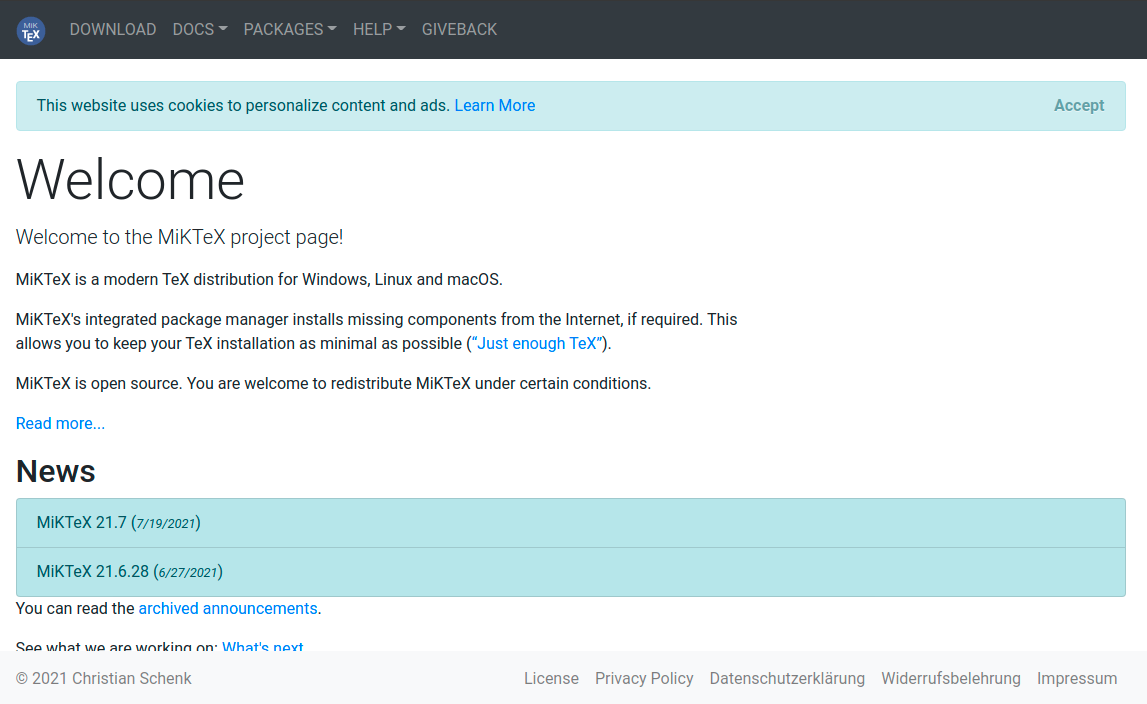
\includegraphics[width=1.0\linewidth 
	%,height=0.4\textheight
	]{Miktex.png}
	\caption[Miktex]{Miktex}
	\label{fig:Miktex}
\end{figure}

\section{Modelos Matemáticos para a Programação Não-Linear}\label{subsection:1}

\hspace{5mm}Determinar a equação de estado que indica o equilíbrio sólido-liquido em um fluido puro a partir da equação molar da energia de \textit{Gibbs}.
\begin{equation}\label{eq:gibbs_2}
\gibbsm^{L}(T,P)=\gibbsm^{S}(T,P)
\end{equation}
como a energia de \textit{Gibbs} é definida por
\begin{equation}\label{eq:gibbs_3}
G\equiv H-TS
\end{equation}
em que $H$ é \textit{entalpia} e $S$ a \textit{entropia}. Derivando a equação \ref{eq:gibbs_3}, obtém-se,
\begin{equation}\label{eq:gibbs_4}
dG=-SdT+VdP
\end{equation}
de tal forma que
\begin{equation}\label{eq:gibbs_5}
\left(\dfrac{\partial G}{\partial T}\right)_{P}=-S
\end{equation}
e 
\begin{equation}\label{eq:gibbs_6}
\left(\dfrac{\partial G}{\partial P}\right)_{T}=V
\end{equation}

Agora integrando a equação \ref{eq:gibbs_6}, obtém-se duas pressões e temperatura constante, obtém-se
\begin{equation}\label{eq:gibbs_7}
G(T_1,P_2)-G(T_1,P_1)=\int_{P_1}^{P_2}VdP
\end{equation}
se o líquido considerado fosse um gás ideal $V^{GI}=\dfrac{RT}{P}$, tal que
\begin{equation}\label{eq:gibbs_8}
G^{GI}(T_1,P_2)-G^{GI}(T_1,P_1)=\int_{P_1}^{P_2}\dfrac{RT}{P}dP
\end{equation}
subtraindo a equação \ref{eq:gibbs_8} de \ref{eq:gibbs_7} obtém-se
\begin{equation}\label{eq:gibbs_9}
[G(T_1,P_2)-G^{GI}(T_1,P_2)]-[G(T_1,P_1)-G^{GI}(T_1,P_1)]=\int_{P_1}^{P_2}\left(V-\dfrac{RT}{P}\right)dP
\end{equation}
sendo assim, considerando $P_1=0$ para todo fluído são gases ideais para que $G(T_1,P=0)=G^{GI}(T_1,P=0)$, pode-se reescrever a equação \ref{eq:gibbs_9}.
\begin{equation}\label{eq:gibbs_10}
G(T,P)-G^{GI}(T,P)=\int_{0}^{P}\left(V-\dfrac{RT}{P}\right)dP
\end{equation}
\cite{Sandlel}

Donde que defini-se a função termodinâmica chamada de \textbf{fugacidade} e indica-se por $f$, definida por
\begin{equation}\label{eq:fugacidade_1}
f=P\mbox{exp}\left\{\dfrac{G(T,P)-G^{GI}(T,P)}{RT}\right\} =P\mbox{exp}\left\{\dfrac{1}{RT}\int_{0}^{P}\left(V-\dfrac{RT}{P}\right)dP\right\}
\end{equation}
em que o coeficiente de fugacidade é definido pela razão $\dfrac{f}{P}$ e é indicada por $\phi$.
\begin{equation}\label{eq:fugacidade_2}
\phi=\dfrac{f}{P}=\mbox{exp}\left\{\dfrac{G(T,P)-G^{GI}(T,P)}{RT}\right\} =\mbox{exp}\left\{\dfrac{1}{RT}\int_{0}^{P}\left(V-\dfrac{RT}{P}\right)dP\right\}
\end{equation}
A função fugacidade existe por uma relação com a energia molar de \textit{Gibbs} para o calculo do equilíbrio de fase. O critério do equilíbrio de duas fases é indicada na equação \ref{eq:gibbs_2} como $\gibbsm^{\mbox{I}}=\gibbsm^{\mbox{II}}$ com a restrição $T$ e $P$ constantes. Dessa equação junto com as equações \ref{eq:fugacidade_1} e \ref{eq:fugacidade_2}. 
\begin{equation}\label{eq:fugacidade_3}
\gibbsm^{GI}(T,P) + RT\ln\dfrac{f^{\mbox{I}}(T,P)}{P} = \gibbsm^{GI}(T,P) + RT\ln\dfrac{f^{\mbox{II}}(T,P)}{P}
\end{equation}
consequentemente a energia de \textit{Gibbs} molar do gás ideal em $T$ e $P$ constante possuem valores iguais, independente da fase utilizada a condição de equilíbrio é indicada
\begin{equation}\label{eq:fugacidade_4}
\ln\dfrac{f^{\mbox{I}}(T,P)}{P} = \ln\dfrac{f^{\mbox{II}}(T,P)}{P}
\end{equation}
em termos de fugacidade
\begin{equation}\label{eq:fugacidade_5}
f^{\mbox{I}}(T,P) = f^{\mbox{II}}(T,P)
\end{equation}
e o coeficiente de fugacidade
\begin{equation}\label{eq:fugacidade_6}
\phi^{\mbox{I}}(T,P) = \phi^{\mbox{II}}(T,P)
\end{equation}
No entanto para fins de cálculo é interessante troca-se a variável $P$ por $V$ uma vez que a pressão é uma constante, da equação \ref{eq:fugacidade_4} e para isso utiliza-se segundo SANDLEL \citeyear{Sandlel}
\begin{equation}\label{eq:fugacidade_7}
dP=\dfrac{1}{\underline{V}}d(P\underline{V})-\dfrac{P}{\underline{V}}d\underline{V}
\end{equation}
em que $\underline{V}$ é o volume molar e mudando a variável de integração obtém-se
\begin{equation}\label{eq:fugacidade_8}
\ln\dfrac{f(T,P)}{P} =\ln\phi = \int_{\underline{V}=\infty}^{\underline{V}}\left[\dfrac{RT}{\underline{V}}-P\right] d\underline{V}-\ln Z+(Z-1)
\end{equation}
quando $Z=\dfrac{P\underline{V}}{RT}$ é chamado de fator de compressão e para obter a equação geral do coeficiente de fugacidade, indicada por
\begin{equation}\label{eq:fugacidade_9}
\ln\dfrac{f(T,P)}{P} =\ln\phi = \int_{\underline{V}=\infty}^{\underline{V}}\left[\dfrac{RT}{\underline{V}}-P\right] d\underline{V}-\ln Z+(Z-1)
\end{equation}
\cite{Sandlel}

Mas para Energia de \textit{Gibbs} em uma mistura em função da temperatura, pressão molar de cada para cada espécie é representada pela diferencial total da função de energia de Gibbs como 
\begin{equation}\label{eq:mistura_1}
dG=-SdT+VdP+\sum_{i=1}^{C}\overline{G}_{i}dN_{i}
\end{equation}
%sandler pg 363 421 (8.2-1)

A energia molar de \textit{Gibbs} é conhecida como \textbf{potencial químico} representada por $\mu_i$, considere as equações para um fluido puro

\begin{equation}
    \frac{1}{N}\left(\frac{\partial G}{\partial P}\right)_{T,N}=\left(\frac{\partial\underline{G}}{\partial P}\right)_{T}=\underline{V}
\end{equation}
,
\begin{equation}
    \frac{1}{N}\left(\frac{\partial G}{\partial T}\right)_{P,N}=\left(\frac{\partial\underline{G}}{\partial T}\right)_{P}=-\underline{S}
\end{equation}
e
\begin{equation}
    \left(\frac{\partial G}{\partial N}\right)_{T,P}=-\underline{G}
\end{equation}

Uma vez que a entalpia pode ser escrita em função da entropia e pressão, segue as equações. 
Por definição $H=U+PV$, tal que
\begin{equation}
    \begin{array}{rcl}
        dH&=&dU+V dP+P dV = T dS - P dV + G dN + V dP + P dV \\
         & = & T dS + V dP + G dN
    \end{array}
\end{equation}
e para um sistema fechado
\begin{equation}
    d\underline{H} = T d\underline{S} + \underline{V} dP
\end{equation}
obtendo
\begin{equation}\label{eq:entalp1}
    \begin{array}{rcl}
        dH & = & \left(\dfrac{\partial H}{\partial P}\right)_{S,N_i}dP + \left(\dfrac{\partial H}{\partial S}\right)_{P,N_i}dS + \displaystyle\sum_{i=1}^{C}\left(\dfrac{\partial H}{\partial N_i}\right)_{P,S,N_{j\neq i}}dN_i  \vspace{3mm}\\
         & = & V dP + T dS + \displaystyle\sum_{i=1}^{C}\left(\dfrac{\partial H}{\partial N_i}\right)_{P,S,N_{j\neq i}}dN_i
    \end{array}
\end{equation}
no entanto, para $H = G + T S$ e Equação \ref{eq:entalp1}, obtém
\begin{equation}\label{eq:entalp2}
    \begin{array}{rcl}
        dH& = & dG + T dS + S dT = -S dT + V dP + \displaystyle\sum  \overline{G}_i dN_i + T dS + S dT\vspace{3mm}\\
          & = & V dP + T dS + \displaystyle\sum  \overline{G}_i dN_i
    \end{array}
\end{equation}

Comparando as Equações \ref{eq:entalp1} e \ref{eq:entalp2}, estabelece
\begin{equation}
    \left(\dfrac{\partial H}{\partial N_i}\right)_{P,S,N_{j\neq i}} = \overline{G}_i = \left(\dfrac{\partial G}{\partial N_i}\right)_{T,P,N_{j\neq i}}
\end{equation}
isto é, a derivada $\left(\dfrac{\partial H}{\partial N_i}\right)_{P,S,N_{j\neq i}}$ é igual a energia parcial molar de Gibbs .

De modo análogo estabelecido
\begin{equation}
    dU = T dS - P dV + \displaystyle\sum_{i}^{C} \overline{G}_i dN_i
\end{equation}
\begin{equation}
    dA = - P dV - S dT + \displaystyle\sum_{i}^{C} \overline{G}_i dN_i
\end{equation}
com
\begin{equation*}
    \overline{G}_i=\left(\dfrac{\partial U}{\partial N_i}\right)_{S,V,N_{j\neq i}}=\left(\dfrac{\partial A}{\partial N_i}\right)_{T,V,N_{j\neq i}}
\end{equation*}
Pode observar que a energia parcial molar de Gibbs assume um papel importante em misturas. 

Agora considere uma função termodinâmica em função de $\theta$ com propriedades molares
\begin{equation*}
    N\underline{\theta} =\sum N_i\overline{\theta}_i
\end{equation*}
derivando pela regra do produto
\begin{equation}\label{eq:ental4}
    d(N\underline{\theta}) = \sum N_i d\overline{\theta}_i + \sum  d\overline{\theta}_i d N_i
\end{equation}
Contudo a função $N\underline{\theta}$ com $T$, $P$ e números de mols.
\begin{equation}\label{eq:ental3}
    d(N\underline{\theta})= N\left(\dfrac{\partial \underline{\theta}}{\partial T}\right)_{P,N_{i}}dT + N\left(\dfrac{\partial \underline{\theta}}{\partial P}\right)_{T,N_{i}}dP+ \sum \overline{\theta}_idN_i
\end{equation}

Subtraindo as Equações \ref{eq:ental3} e \ref{eq:ental4} obtém-se a  \textbf{equação generalizada Gibbs-Duhem}.
\begin{equation}
    \displaystyle\sum_{i=1}^{C}N_id\overline{\theta}_i|_{T,P}=0
\end{equation}
e a equação de Gibbs-Duhem com $T$ e $P$ constantes.
\begin{equation}
    \displaystyle\sum_{i=1}^{C}x_id\overline{\theta}_i|_{T,P}=0
\end{equation}

Para misturas binárias 
\begin{equation}
    \displaystyle\sum_{i=1}^{2}x_i\left(\dfrac{\partial \underline{\theta}_1}{\partial x_1}\right)_{T,P}dx_1=0
\end{equation}

Determinando a equação de Gibbs-Duhem para misturas binárias com $T$ e $P$ constantes.

\begin{equation}
   x_1\left(\dfrac{\partial \underline{G}_1}{\partial x_1}\right)_{T,P}+ x_2\left(\dfrac{\partial \underline{G}_2}{\partial x_1}\right)_{T,P}=0
\end{equation}
usando $x_2=1-x_1$ e $dx_2=-dx_1$.

%Modelagerm_Matemática
\chapter{MATERIAIS E MÉTODOS}
\label{Material_metodo}

\section{Materiais}
\hspace{0.5cm} O trabalho tem caráter teórico e computacional com aplicação de técnicas de otimização matemática de programação não-linear, implementado no \textit{software} $GAMS$ (\textit{General Algebric Model System}), planilha eletrônica, \textit{software} Geogebra, \textit{PyCharm}.

\section{Métodos}

\hspace{0.5cm} Para o determinar o equilíbrio de fase sólido-líquido, foram aplicados os modelos termodinâmicos, por meio de cálculos pode-se determinar coeficientes ligados diretamente com a Energia livre de Gibbs.  \cite{Rocha2009a,Costa2007}

Segundo ROCHA \citeyear{Rocha2009a}, o diagrama de fase sólido-líquido para misturas binárias pode ser encontrado pela minimização da energia de Gibbs. O método para determinar o diagrama de fase sólido-líquido é capaz de incluir o número de componentes ($NC$) desejado, o valor de componentes para esse trabalho é de $NC=2$, com possibilidade futura de aplicações em misturas de mais componentes. A condição necessária para o mínimo, de componentes e produto, é dada pela convexidade do problema. Mas uma suposição implícita usada aqui no modelo é de que existe apenas uma fase líquida. Portanto para um modelo geral de atividade líquida deve ter uma análise cuidadosa, pois em modelos não-convexos, podem ser verificadas existências de outras possibilidades de equilíbrio, do tipo líquido-líquido-sólido, por exemplo. 

\subsection{Modelo geral para fase líquida}

\hspace{0.5cm} A equação abaixo indicada por $B_{i}$ (\ref{eq:Fugacidade_1}) é o parâmetro relativo a fugacidade nas fases líquida e sólida do componente $i$, em que $\Delta h_{fi}$ representa entalpia de fusão para o componente $i$, $T_{fi}$ é a temperatura de fusão do componente $i$.
\begin{equation}\label{eq:Fugacidade_1}
B_{i}=\frac{\Delta h_{fi}}{R\cdot T_{fi}}\cdot\left(\frac{T_{fi}}{T}-1\right)
\end{equation}

Logo é possível determinar expressões para a temperatura em função da fração molar, que na maioria dos modelos líquidos exigirá um procedimento interativo.

Existem três regiões possíveis no diagrama de fases $T\times x_{1}$ para o ESL:  Região I é aquela em que a fase sólida é o componente 2 e representada pela equação e a respectiva restrição (Eq. \ref{eq:Regiao_I_1} e \ref{eq:Regiao_I_2}); A região II é aquela em que a fase sólida é o componente 1 e representada pelas equação e a respectiva restrição (Eq. \ref{eq:Regiao_II_1} e \ref{eq:Regiao_II_2}); A região III, se existir, é aquela em que a fase sólida é o composto  e representada pelas equação e respectivas restrições (Eqs. \ref{eq:Regiao_III_1}, \ref{eq:Regiao_III_2} e \ref{eq:Regiao_III_3}).

\subsubsection{Região I}
\begin{equation}\label{eq:Regiao_I_1}
T=\frac{\Delta h_{f2}}{\frac{\Delta h_{f2}}{T_{f2}}-R\cdot\ln[(1-x_{1})\gamma_{2}^{l}]}
\end{equation}
limitado pelas restrições:
\begin{equation}\label{eq:Regiao_I_2}
-R\cdot T\cdot[B_{1}+\ln x_{1}]-R\cdot T\cdot\ln\gamma_{1}^{l}\geq\max\left\{0,\frac{1}{v_1}\cdot\Delta G_{R}^{\circ} \right\}
\end{equation}

\subsubsection{Região II}
\begin{equation}\label{eq:Regiao_II_1}
T=\frac{\Delta h_{f1}}{\frac{\Delta h_{f1}}{T_{f1}}-R\cdot\ln[(x_{1})\gamma_{1}^{l}]}
\end{equation}
limitado pelas restrições:
\begin{equation}\label{eq:Regiao_II_2}
-R\cdot T\cdot[B_{2}+\ln(1- x_{1})]-R\cdot T\cdot\ln\gamma_{2}^{l}\geq\max\left\{0,\frac{1}{v_2}\cdot\Delta G_{R}^{\circ} \right\}
\end{equation}

\subsubsection{Região III}
\begin{equation}\label{eq:Regiao_III_1}
T=\frac{\nu_{1}\cdot\Delta h_{f1} + \nu_{2}\cdot\Delta h_{f2} + \Delta G_{R}^{\circ}}{\nu_{1}\cdot\frac{\Delta h_{f1}}{T_{f1}}+\nu_{2}\cdot\frac{\Delta h_{f2}}{T_{f2}}-\nu_{1}\cdot R\cdot\ln[(x_{1})\gamma_{1}^{l}]-\nu_{2}\cdot R\cdot\ln[(1-x_{1})\gamma_{2}^{l}]}
\end{equation}
limitado pelas restrições:
\begin{equation}\label{eq:Regiao_III_2}
0\leq-R\cdot T\cdot[B_{1}+\ln x_{1}]-R\cdot T\cdot \ln\gamma_{1}^{l}\leq\max\left\{0,\frac{1}{\nu_1}\cdot
\Delta G_{R}^{\circ} \right\}
\end{equation}
\begin{equation}\label{eq:Regiao_III_3}
0\leq-R\cdot T\cdot[B_{2}+\ln(1- x_{1})]-R\cdot T\cdot\ln\gamma_{2}^{l}\leq\max\left\{0,\frac{1}{\nu_2}\cdot
\Delta G_{R}^{\circ} \right\}
\end{equation}

As equações  não são realmente explícitos em $T$, pois $\gamma_{i}^{l}$ são em função de $T$ e $x_{i}^{l}$.

\subsection{Modelo de Margules Simétrico para fase líquida}

Será usado nesse trabalho a fase líquida modelada pela equação (Eq. \ref{eq:Margules_1}) considerando o modelo de Margules com 2-sufixo:
\begin{equation}\label{eq:Margules_1}
R\cdot T\cdot\ln\gamma_{i}^{l}=\frac{1}{2} \cdot\sum_{j=1}^{NC}\sum_{k=1}^{NC}\left( A_{ij}+A_{ji}-A_{jk}\right) \cdot x_{j}^{l}\cdot x_{k}^{l}
\end{equation}

Considerando que $A_{ii}=0$ e $A_{ij}=A_{ji}$, a energia livre de Gibbs para problemas com uma mistura binária em uma fase líquida pode-se escrever:

\begin{equation}
\begin{split}
G=(\eta_{1}^{0}\cdot\nu_{1}^{S,\circ}+\eta_{2}^{0}\cdot\nu_{2}^{S,\circ})+ \eta_{p}^{0}\cdot\Delta G_{R}^{\circ}+ \eta_{p}^{S}\cdot\Delta G_{R}^{\circ} +R\cdot T\\\cdot \left[\eta_{1}^{l} \left( B_{1}+\ln\eta_{1}^{l}-\ln(\eta_{1}^{l} +\eta_{2}^{l} )\right)+\eta_{2}^{l}\left( B_{2}+\ln\eta_{2}^{l}-\ln(\eta_{1}^{l} +\eta_{2}^{l} )\right) \right]
\\+\frac{A_{12}\eta_{1}^{l}\eta_{2}^{l}}{\eta_{1}^{l}+\eta_{2}^{l}}
\end{split}
\end{equation}

Conforme o formulado, possui apenas um ponto mínimo se o problema for restrito a $\dfrac{A_{12}}{R}\cdot T\leq2$, de forma que a condição de Kutn-Tucker sejam necessárias e suficientes para o mínimo global \cite{Edgar2001}.

Dessa forma usando as equação (\ref{eq:Regiao_I_1}), (\ref{eq:Regiao_II_1}), (\ref{eq:Regiao_III_1}) e (\ref{eq:Margules_1}), determinam as equações explícitas para a temperatura $T$, em função da fração molar do componente 1 da fase $x_ 1$.

\subsubsection{Região I}

\begin{equation}
T=\frac{\Delta h_{f2}+A_{12}\cdot x_{1}^{2}}{\frac{\Delta h_{f2}}{T_{f2}} -R\cdot\ln(1-x_{1})}
\label{equa_5}
\end{equation}

limitado pelas restrições:

\begin{equation}
-R\cdot T\cdot[B_{1}+\ln x_{1}]-A_{12}\cdot(1-x_{1})^{2}\geq\max\left\{0,\frac{1}{\nu_1}\cdot\Delta G_{R}^{\circ} \right\}
\label{limite_5}
\end{equation}

\subsubsection{Região II}

\begin{equation}
T=\frac{\Delta h_{f1}+A_{12}\cdot (1-x_{1})^{2}}{\frac{\Delta h_{f1}}{T_{f1}} -R\cdot\ln x_{1}}
\label{equa_6}
\end{equation}

limitado pelas restrições:

\begin{equation}
-R\cdot T\cdot[B_{2}+\ln (1-x_{1})]-A_{12}\cdot x_{1}^{2}\geq\max\left\{0,\frac{1}{\nu_2}\cdot\Delta G_{R}^{\circ} \right\}
\label{limite_6}
\end{equation}

\subsubsection{Região III}

\begin{equation}
T=\frac{\nu_{1}\cdot\Delta h_{f1} + \nu_{2}\cdot\Delta h_{f2}+\nu_{1}\cdot A_{12}\cdot(1-x_{1})^{2}+ \nu_{2}\cdot A_{12}\cdot x_{1}^{2} + \Delta G_{R}^{\circ}}{\nu_{1}\cdot\frac{\Delta h_{f1}}{T_{f1}}+\nu_{2}\cdot\frac{\Delta h_{f2}}{T_{f2}}-\nu_{1}\cdot R\cdot\ln x_{1}-\nu_{2}\cdot R\cdot\ln(1-x_{1})}
\label{equa_7}
\end{equation}
limitado pelas restrições:
\begin{equation}
0\leq-R\cdot T\cdot[B_{1}+\ln x_{1}]-A_{12}\cdot (1+x_{1})^{2}\leq\max\left\{0,\frac{1}{\nu_1}\cdot
\Delta G_{R}^{\circ} \right\}
\label{limite_7}
\end{equation}
\begin{equation}
0\leq-R\cdot T\cdot[B_{2}+\ln(1- x_{1})]-A_{12}\cdot x_{1}^{2}\leq\max\left\{0,\frac{1}{\nu_2}\cdot
\Delta G_{R}^{\circ} \right\}
\label{limite_8}
\end{equation}

\subsection{Modelo de Margules Simétrico}

Para o desenvolvimento do algoritmo para a transição de fase, considere a fase sólida como a ideal que é determinada por SLAUGHTER e
DOHERTY \citeyear{Douglas1995} e a fase liquida modelada representada por \textit{Margules}  2-sufixo.\cite{Rocha2009a}

Para isso a função fugacidade é definida por:
\begin{equation}\label{eq:Margules_3}
d\mu_{i}(T,P)=d\overline{G}_i=RTd\ln(\hat{f}_i)
\end{equation}
em que $T$ é uma constante e aplicando a integração, obtemos
\begin{equation}\label{eq:Margules_4}
\mu_{i}(T,P)=\mu^{\circ}_{i}(T)+RT\ln\left(\dfrac{\hat{f}_i}{f^{\circ}_{i}}\right)
\end{equation}
para o gás ideal a 1$atm$, obtemos $f^{\circ}_{i}=1$ e para um composto puro $f^{\circ}_{i}=f^{\circ}_{\ell,i}$. \cite{Rocha2009a}

Energia Livre de \textit{Gibbs} total do sistema e dada por
\begin{equation}\label{eq:Gibbs_1}
G=\sum_{k=1}^{NF}\sum_{i=1}^{NC}\eta_{i}^{k}\cdot\mu_{i}^{k}
\end{equation}
substituindo a equação \ref{eq:Margules_4} em \ref{eq:Gibbs_1}, obtém:
\begin{equation}\label{eq:Gibbs_2}
G=\sum_{k=1}^{NF}\sum_{i=1}^{NC}\eta_{i}^{k}\cdot\mu_{i}^{\circ}+RT\sum_{k=1}^{NF}\sum_{i=1}^{NC}\eta_{i}^{k}\ln\left(\dfrac{\hat{f}_i}{f^{\circ}_{i}}\right)
\end{equation}
minimizando $G$ em relação à $\eta_{i}^{k}$ em que $P$ e $T$ são constante, isto é
\begin{equation}\label{eq:Gibbs_3}
G=\sum_{k=1}^{NF}\sum_{i=1}^{NC}\eta_{i}^{k}\ln\left(\dfrac{\hat{f}_i}{f^{\circ}_{i}}\right)
\end{equation}
\cite{Rocha2009a}.

Será usado nesse trabalho a fase líquida modelada pela equação (Eq. \ref{eq:Margules_2}) considerando o modelo de Margules com 2-sufixo:
\begin{equation}\label{eq:Fugacidade_2}
\hat{f}_i^{k}=f_{i}^{\circ}x_i^{k}\gamma_i^{k}
\end{equation}
em que $f_{i}^{\circ}$ representa a fugacidade na componete $i$ para composto puro e na fase $k$.

\subsection{Margules 2-sufixos para fase liquida}

Para a fase líquida, usamos o modelo de \textit{Margules} Assimétrico
\begin{equation}
\underline{G}^{ex}=RT\sum_{i-1}^{NC}x_i\ln(\gamma_{i})=\sum_{k=1}^{NF}\sum_{i=1}^{NC}A_{ij}x_ix_j
\end{equation}
para implementação no \textit{GAMS}
\begin{equation}\label{eq:margules_6}
G=\sum_{i=1}^{NC}\left[\eta_{i}^{\ell}\left(B_i+\ln\eta_i^\ell -\ln\sum_{j=1}^{NC}\eta_{i}^\ell+\dfrac{\displaystyle\sum_{j=1}^{NC}A_{ij} \eta_{j}^\ell}{2RT\displaystyle\sum_{i=1}^{NC}\eta_{i}^\ell}\right)\right]
\end{equation}
\cite{Rocha2009a}.

E \textit{Margules} Simétrico para o \textit{GAMS} usa \textit{Margules} 2-sufixo em que $A_{ii}=0$ e $A_{ij}=A_{ji}$ em a equação \ref{eq:margules_6} é dada por
\begin{equation}
G=\sum_{i=1}^{NC}\left[\eta_{i}^{\ell}\left(B_i+\ln\eta_i^\ell -\ln\sum_{j=1}^{NC}\eta_{i}^\ell\right)\right]+\dfrac{1}{RT}\dfrac{\displaystyle\sum_{i<j}A_{ij} \eta_{i}^\ell  \eta_{j}^\ell }{2RT\displaystyle\sum_{i=1}^{NC}\eta_{i}^\ell}
\end{equation}
em que $B_{i}$ é o parâmetro do modelo para determinar o mínimo de \textit{Gibbs}.\cite{Rocha2009a}

\subsection{Wilson}
A equação de \textit{Wilson} é representada por
\begin{equation}
\ln\gamma_{i}=-\ln(x_i+x_j\Lambda_{ij})+x_j\left[ \dfrac{\Lambda_{ij}}{x_i+x_j\Lambda_{ij}}-\dfrac{\Lambda_{ji}}{x_i\Lambda_{ji}+x_j}\right]
\end{equation}
\begin{equation}
\ln\gamma_{j}=-\ln(x_j+x_i\Lambda_{ji})+x_j\left[ \dfrac{\Lambda_{ji}}{x_j+x_i\Lambda_{ji}}-\dfrac{\Lambda_{ij}}{x_i\Lambda_{ij}+x_j}\right]
\end{equation}

\subsection{Ponto eutético e ponto peritético}

Como $\nu_{1}<0$ e $\nu_{2}<0$ se $\Delta G_{R}^{\circ}$ a Região III não existe. Neste caso, seja encontrada a composição do ponto eutético é determinado pela intersecção das equações (\ref{equa_5}) e (\ref{equa_6}):

\begin{equation}
\frac{\Delta h_{f2}+A_{12}\cdot x_{1}^{2}}{\frac{\Delta h_{f2}}{T_{f2}} -R\cdot\ln(1-x_{1})}=\frac{\Delta h_{f1}+A_{12}\cdot (1-x_{1})^{2}}{\frac{\Delta h_{f1}}{T_{f1}} -R\cdot\ln x_{1}}
\end{equation}

onde cada uma tem as restrições (\ref{limite_5}) e (\ref{limite_6}).

Do mesmo modo $\nu_{1}<0$ e $\nu_{2}<0$, se $\Delta G_{G}^{\circ}<0$ a Região III existe, de modo que existem dois pontos:

\begin{equation}
\frac{\Delta h_{f2}+A_{12}\cdot x_{1}^{2}}{\frac{\Delta h_{f2}}{T_{f2}} -R\cdot\ln(1-x_{1})}=\frac{\nu_{1}\cdot\Delta h_{f1} + \nu_{2}\cdot\Delta h_{f2}+\nu_{1}\cdot A_{12}\cdot(1-x_{1})^{2}+ \nu_{2}\cdot A_{12}\cdot x_{1}^{2} + \Delta G_{R}^{\circ}}{\nu_{1}\cdot\frac{\Delta h_{f1}}{T_{f1}}+\nu_{2}\cdot\frac{\Delta h_{f2}}{T_{f2}}-\nu_{1}\cdot R\cdot\ln x_{1}-\nu_{2}\cdot R\cdot\ln(1-x_{1})}
\label{equa_8}
\end{equation}
e 
\begin{equation}
\frac{\Delta h_{f1}+A_{12}\cdot (1-x_{1})^{2}}{\frac{\Delta h_{f1}}{T_{f1}} -R\cdot\ln x_{1}}=\frac{\nu_{1}\cdot\Delta h_{f1} + \nu_{2}\cdot\Delta h_{f2}+\nu_{1}\cdot A_{12}\cdot(1-x_{1})^{2}+ \nu_{2}\cdot A_{12}\cdot x_{1}^{2} + \Delta G_{R}^{\circ}}{\nu_{1}\cdot\frac{\Delta h_{f1}}{T_{f1}}+\nu_{2}\cdot\frac{\Delta h_{f2}}{T_{f2}}-\nu_{1}\cdot R\cdot\ln x_{1}-\nu_{2}\cdot R\cdot\ln(1-x_{1})}
\label{equa_10}
\end{equation}

Onde $T$ mais baixo é o ponto eutético, enquanto o outro é o ponto peritético.

A equação (\ref{equa_8}) pode ser reorganizada para:

\begin{equation}
\frac{\Delta h_{f2}+A_{12}\cdot x_{1}^{2}}{\frac{\Delta h_{f2}}{T_{f2}} -R\cdot\ln(1-x_{1})}=\frac{\Delta h_{f1}+A_{12}\cdot(1-x_{1})^{2} +\frac{1}{\nu_{1}}\cdot\Delta G_{R}^{\circ}}{\frac{\Delta h_{f2}}{T_{f2}} -R\cdot\ln (1-x_{1})}
\label{equa_9}
\end{equation}

a equação (\ref{equa_9}) possui os mesmos limites de restrições de (\ref{limite_5}) e (\ref{limite_7}).

E reescrevendo a equação (\ref{equa_10}):
\begin{equation}
\frac{\Delta h_{f1}+A_{12}\cdot (1-x_{1})^{2}}{\frac{\Delta h_{f1}}{T_{f1}} -R\cdot\ln(x_{1})}=\frac{\Delta h_{f2}+A_{12}\cdot x_{1}^{2} +\frac{1}{\nu_{2}}\cdot\Delta G_{R}^{\circ}}{\frac{\Delta h_{f2}}{T_{f2}} -R\cdot\ln (1-x_{1})}
\label{equa_11}
\end{equation}

em que a equação (\ref{equa_11}) tem as mesmas restrições de (\ref{limite_6}) e (\ref{limite_8}).

\subsection{Aplicações das ferramentas computacionais}
\subsubsection{Geogebra}

Neste trabalho foi utilizado \textit{Geogebra Clássico 5}  uma versão \textit{offline}, com uma interface mais pragmática que traz maior confiança no trabalho, Figura \ref{fig:12}, o motivo de usar essa ferramenta para coleta de dados de DSC nos artigos pesquisados, já que determinados artigos não possuem os dados em forma de tabela.
\begin{figure}[H]
	\centering
	\includegraphics[width=0.9\linewidth 
	%,height=0.4\textheight
	]{dados/figuras/Geogebra_2.png}
	\caption[Interface gráfica do Geogebra]{Interface gráfica do Geogebra}
	\label{fig:12}
\end{figure}

A finalidade do Geogebra tem o propósito a coleta dos pares ordenados  (\textit{misturas;temperatura}), já que alguns dados de misturas e temperaturas não são fornecidas em forma de tabela, como para o sistema hexadecanol e ácido mirístico, a grande preocupação de coletar os dados a partir do diagrama é adquirir esse valores de forma precisa com base nos artigos, o procedimento para obtenção dos dados segue os passos: 
\begin{itemize}
    \item Tirar a foto com a tecla \textit{print screen} ou \keystroke{PrtScr} (a simplificação dos teclados pode variar muito de marca e modelo de teclado), para agilizar é de bom senso usar as tecla de atalho \Shift$+$\keystroke{PrtScr} para capturar apenas a área desejada e manter a qualidade da imagem.
    \item Utilizar um aplicativo de imagem para alterar escala do eixos das abscissa e ordenada, para que os eixos das coordenadas do Geogebra coincida com os eixos das coordenadas do artigo, com a finalidade de que os pares ordenados sejam mais precisa. Para esse trabalho o aplicativo \textit{Kolourpaint}\footnote{Se encontra no site \url{https://apps.kde.org/pt-br/kolourpaint/}, até o momento esse versão é para versões Linux.} foi utilizado pela interface gráfica simples, fácil de se manusear e de código aberto.
    \item Na Figura \ref{fig:DSC_Hexadec+Miristi} mostra o diagrama de fase no Geogebra como imagem de fundo, para isso na \textbf{barra de ferramentas} clique em \textbf{Editar}, \textbf{Inserir imagem de} e \textbf{Arquivo}, ajustar a imagem conforme a escala dos eixos das coordenadas, depois vá em \textbf{Exibir} marque a opção \textbf{Planilha}, desse modo podemos coletar a informação em uma planilha.
    \item Nas coordenadas foi usada uma aproximação de 10 casas decimais, para modificar vá em \textbf{barra de ferramentas} clique em \textbf{Arredondamento} e selecione a aproximação que melhor convém.
    \item Para a coleta automática dos pares ordenados, primeiro inserir todos os pontos e posiciona-los nas respectivas posições da mistura e temperatura, segundo na \textbf{barra de ferramentas} da planilha selecione \textbf{Lista de pontos}, terceiro criada a lista de pontos na \textbf{Janela de Álgebra} clique com botão direito do mouse na lista e vá em \textbf{propriedades} e em \textbf{Definição} adicione os pontos, em quarto clique com botão direito do mouse e selecione \textbf{Gravar para Planilha de Cálculos} e finalmente na planilha clique sobre o ponto vermelho (\textit{rec}) para gravar os valores.
\end{itemize}
\begin{figure}[H]
	\centering
	\includegraphics[scale=0.3]{DSC_Hexadec+Miristi}
	\caption[Geogebra coleta de pares ordenados]{Coleta de pares ordenados}
	\label{fig:DSC_Hexadec+Miristi}
\end{figure}
Conforme a Figura \ref{fig:DSC_Hexadec+Miristi} com todos os procedimentos acima, obtém-se na coluna à esquerda os pares ordenados e na coluna à direita os dados disponíveis na planilha eletrônica.

Recomenda-se paciência no ajuste da escala, pois esse ajuste da imagem com a escala é um procedimento tedioso, requer paciência, levando em varias vezes o mesmo procedimento.

\subsubsection{Planilha eletrônica}
A planilha eletrônica foi utilizada como banco de dados, para armazenar os pares ordenados da mistura e temperatura do DSC, uma forma de armazenar e organizar os dados como, temperatura de fusão, entalpia, cálculos de conversões de unidades de medidas com Celcius para kelvin e  de kilo joule para quilo, o recurso de transposição de dados, isto é, troca os dados de linhas para colunas  o algoritmo da biblioteca R trabalhar com os dados e armazenar dados de caloria máxima obtida diante o cálculo das Temperaturas das referidas regiões classificadas como I, II e III. 

\subsubsection{\textit{GAMS}}
O \textit{software} \textit{GAMS} foi usado para determinar as temperaturas de fusão com as determinadas misturas binárias para os modelos termodinâmicos Margules Simétrico, Margules Assimétrico e Wilson, com o método matemático de  programação não linear, com o solver CONOPT com solução satisfatória.

\subsubsection{\textit{PyCharm} e \textit{R}}
No desenvolvimento deste trabalho ambos \textit{softwares} foram utilizados para coletar os dados da planilha e plotar os gráficos. O algoritmo foi escrito em \textit{R} e compilado pelo \textit{PyCharm}. Todos os dados de mistura e temperatura se encontram no repositório do \textit{GitHub}, junto com os algoritmos dos diagramas e coeficiente de determinação.
 %Materiais_métodos
\chapter{RESULTADOS E DISCUSSÕES}

Os resultados obtidos, a partir do desenvolvimento de  6 sistemas de misturas binárias, foram subdivididos em subitens nos estudos de casos. Esses estudos contemplam misturas de ácidos graxos e álcoois, sendo a aplicação da modelagem matemática utilizada inovadora neste último grupamento funcional.

Para comparar os resultados obtidos,  gráficos foram construídos, gerando diagramas de fases sólido-líquido, evidenciados pelas características mais relevantes: linha \textit{liquidus}, ponto eutético e/ou ponto peritético, a partir da aplicação dos  modelos MA, MS e Wilson, já descritos anteriormente.

A escala de cada diagrama de fase das misturas binárias são distintas, pelo fato de que cada ácido graxo ou álcool possui ponto de fusão distintos como podemos verificar nas seções \ref{sec:1} até \ref{sec:6}.

A partir dos dados experimentais coletados do referencial teórico utilizado determinados pela técnica de DSC, o DSC é uma técnica com a finalidade de encontrar os limites de fase, a partir de medidas dos efeitos térmicos durante o processo de mudança de fase.

A metodologia estatística de $R^2$ (coeficiente de determinação) foi aplicada, para determinar o percentual em que a metodologia de DSC está representada pelo algoritmo, com os modelos MA, MS e \textit{Wilson}.

\section{Estudos de casos.}

\subsection{Sistema 1: Ácido Mirístico e Ácido Esteárico}\label{sistema1}
Com a aplicação da modelagem matemática na seção \ref{subsection:1}, cujo desenvolvimento resultou em um modelo de PNL, foi possível obter o diagrama de fase sólido-líquido para esse sistema.

Na Figura \ref{fig:3} o diagrama de fase foi determinado pelos modelos termodinâmicos \textit{MA}, \textit{MS} e \textit{Wilson} implementado no \textit{GAMS} e o gráfico gerado pelo \textit{PyCharm} com biblioteca do \textit{R}. Os dados experimentais comparativos foram obtidos por COSTA 2009 por experimentos com o método de DSC.
\begin{figure}[H]
	\centering
	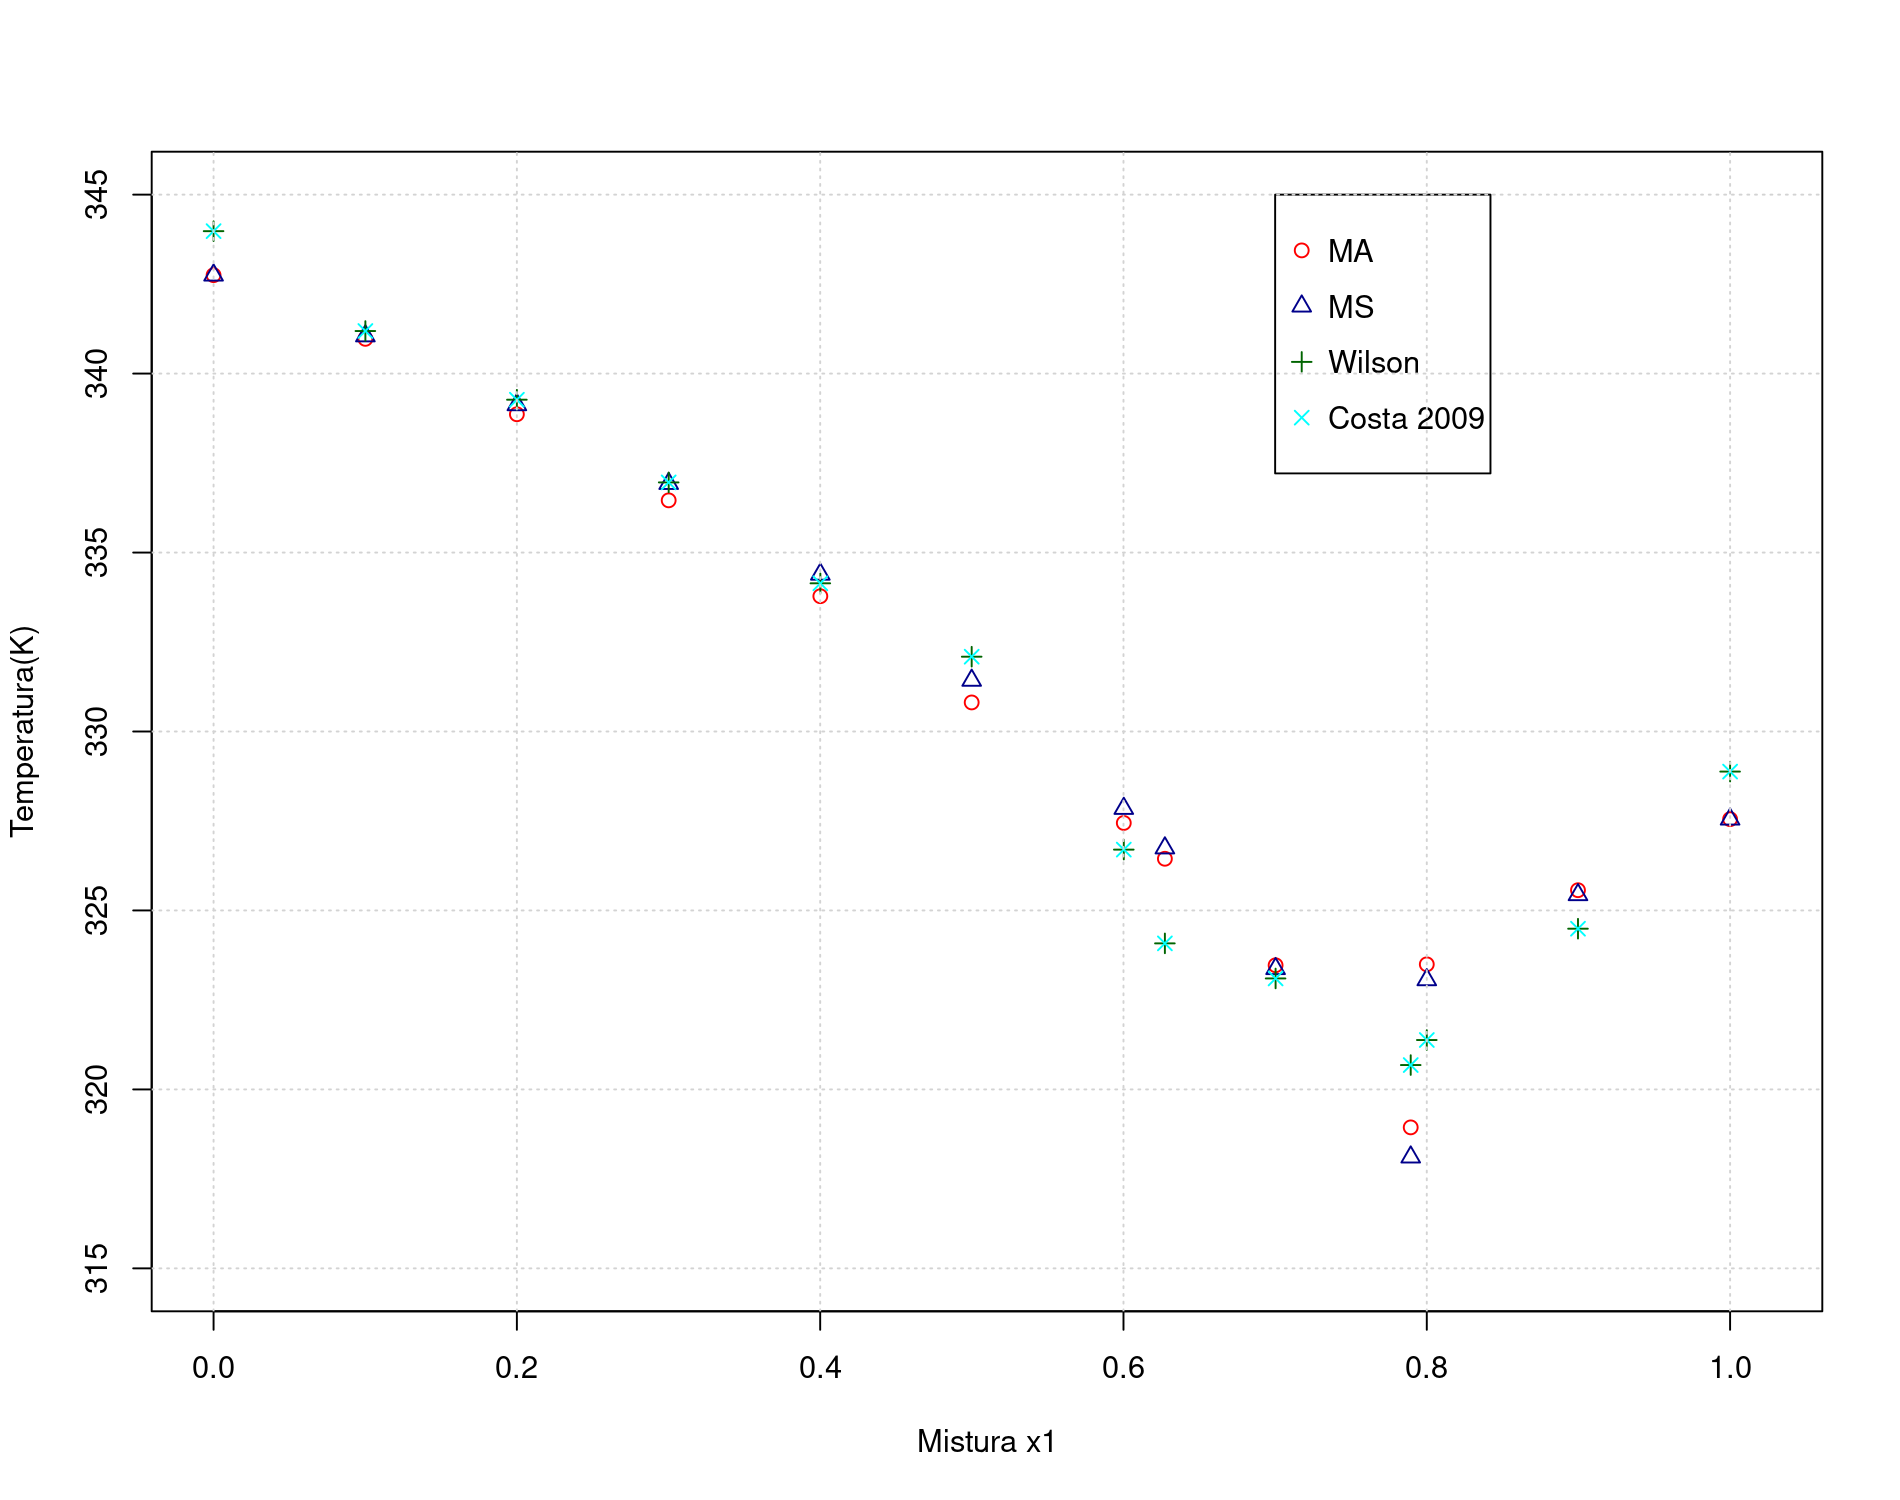
\includegraphics[width=1.06\linewidth 
	%,height=0.4\textheight
	]{dados/figuras/Miristico_estearico.png}
	\caption[Diagrama do equilíbrio sólido-líquido para mistura Ácido Mirístico e Ácido Esteárico]{Diagrama do equilíbrio sólido-líquido para mistura Ácido Mirístico(1) e Ácido Esteárico(2) (\textit{PyCharm}/$R$)}
	\label{fig:3}
\end{figure}

A partir do diagrama de fases obtido, evidencia-se a formação da linha \textit{liquidus} praticamente sobreposta aos dados experimentais comparativos, e entre os modelos termodinâmicos estudados, até a composição aproximada de 50\% da mistura ácido mirístico e ácido palmítico. Após essa medida intermediária, verifica-se maior distanciamento das técnicas computacionais aplicadas, comparada ao dados de DSC, porém mantém-se a inclinação desejada, com a percepção da formação do ponto eutético próximo a composição 0,6 e uma outra visualização de mudança de inclinação próximo a composição 0,8, referindo-se a presença do ponto peritético. Vale ressaltar a relevância teórico/computacional da sensibilidade e robustez de modelos termodinâmicos serem capazes de prever tais pontos específicos de transição, principalmente o ponto peritético.

%\begin{comment}
%\subsection{Sistema 2: Ácido Palmítico e Ácido Esteárico} \label{sistema2}
%Aqui também a aplicação da modelagem matemática já citada, cujo desenvolvimento resultou em um modelo de \textit{PNL}, foi possível obter o diagrama de fase sólido-líquido para esse sistema.
%Na Figura \ref{fig:4} o diagrama de fase foi determinado pelos modelos termodinâmicos \textit{MA}, \textit{MS} e \textit{Wilson} implementado no \textit{GAMS} e o gráfico gerado pelo \textit{PyCharm} com biblioteca do \textit{R}.
%\begin{figure}[H]
%	\centering
%	\includegraphics[width=1.06\linewidth 
	%,height=0.4\textheight
%	]{dados/figuras/Palmitico_estearico_DSC.png}
%	\caption[Diagrama do equilíbrio sólido-líquido para mistura Ácido Palmítico e Ácido Esteárico]{Diagrama do equilíbrio sólido-líquido para mistura Ácido Palmítico(1) e Ácido Esteárico(2) (\textit{PyCharm}/\textit{R}) Autor.}
%	\label{fig:4}
%\end{figure}
%\end{comment}


\subsection{Sistema 2: Ácido Palmítico e Ácido Esteárico}\label{sistema3}



Com a definição dos pares ordenados para composição de mistura e temperatura,  foi possível obter a linha \textit{liquidus} praticamente sobreposta aos dados experimentais comparativos próximos as composições de substância pura, em que visualmente o modelo de Margules Assimétrico tem maior proximidade aos dados experimentais. Quanto a inclinação das curvas definidas pelas regiões calculadas, são apresentadas inclinações equivalentes aos dados experimentais.  Ressalta-se a importância de modelos teórico/computacionais apresentarem, pela aplicação dos modelos termodinâmicos adequados, a capacidade de predição de formação do ponto eutético.




\section{Coeficiente de Determinação}

O Coeficiente de Determinação ou $R^2$ foi aplicado como técnica comparativa entre os resultados obtidos da literatura ao utilizar experimentalmente a técnica de DSC (Calorimetria exploratória diferencial) aos modelos MA, MS e Wilson em cada um dos sistemas, para averiguação da representatividade de cada modelo. Dessa forma considerados os dados de DSC como $VD$ (variável dependente) ou variável resposta e dos modelos aplicados como $VI$ (variável independente) ou variável de regressão. O $R^2$ fornece um valor em percentagem ou valor decimal cuja a interpretação é, quantos de $VD$ é explicada por $VI$ ou quantos que $VI$ tem influencia sobre $VD$, isto é, $R^2$ é a proporção da variação de $VD$ explicada pela variação de $VI$. 

A propriedade do coeficiente de determinação é que:
\begin{itemize}
    \item $R^2\in [0;1]$
    \item $R^2=1$, $VD$ é explicada pela variação de $VI$ em 100\%
    \item $R^2=0$, $VI$ não tem influencia sobre $VD$.
\end{itemize}

O valor do $R^2$ é calculado pela fórmula
\begin{equation}
    R^2=\frac{\left(\displaystyle\sum_{i=1}^{n}x_i\cdot y_i-n\cdot\overline{x}\cdot\overline{y}\right)^2}{\left(\displaystyle\sum_{i=1}^{n}x_i^2-n\cdot\overline{x}^2\right)\times\left(\displaystyle\sum_{i=1}^{n}y_i^2-n\cdot\overline{y}^2\right)}
\end{equation}
em que $n$ quantidade de elementos da variável $VD$ ou $VI$, $x_i\in VI$ e $y_i\in VD$.
\begin{equation}
    \overline{x}=\frac{\displaystyle\sum_{i=1}^{n}x_i}{n}
\end{equation}
e
\begin{equation}
    \overline{y}=\frac{\displaystyle\sum_{i=1}^{n}y_i}{n}
\end{equation}

%\begin{center}
    %Coeficiente de determinação da variável dependente  técnicas de %DSC e variáveis independentes MA, MS ou Wilson
%\end{center}
\begin{table}[H]
    \caption{Coeficiente de Determinação}
    \centering
    \begin{tabular}{l|p{3cm}p{3cm}p{3cm}}
    %\multicolumn{4}{c}{\textbf{Coeficiente de determinação da variável dependente  técnicas de DSC e variáveis}}  \\ 
    %\multicolumn{4}{c}{\textbf{independentes MA, MS ou Wilson}} \\ 
    \hline
         & $R^2$ MA & $R^2$ MS & $R^2$ Wilson \\
    \hline
    Ac. Mirístico e Ac. Esteárico  & 0.9756  & 0.9706 & 0.9708 \\
    Ac. Palmítico e Ac. Esteárico  & 0.9699  & 0.8005 & 0.7040 \\
    %Ac. Palmítico e Ac. Esteárico  & 0.4955  & 0.5355 & 0.5057 \\
    Hexadecanol e Ac. Mirístico  & 0.2427  & 0.2328 & 0.2133 \\
    Hexadecanol e Tetradecanol  & 0.9804  & 0.9310 & 0.9887 \\
    Ac. Esteárico e Ac. Linoleico  & 0.1483  & 0.5592 & 0.8745 \\
    Ac. Palmítico e Ac. Linoleico  & 0.7490  & 0.5602 & 0.0000 \\
    \end{tabular}
    \label{tab:1}
\end{table}

 %Resultados
%% RESULTADOS-------------------------------------------------------------------

\chapter{Resultados Esperados}

De acordo com os objetivos propostos, foram definidos os compostos carbônicos capazes de compor as misturas carbônicas, como ácidos graxos e álcoois para que haja a identificação e definição dos diagramas de fases, utilizando a modelagem matemática e termodinâmico que calculam e encontram os critérios que identificam o equilíbrio de fase sólido-liquido. De tal forma que o uso teórico e computacional é vital para o trabalho, para aplicação dos métodos e resultados sustentáveis.

Após determinação dos sistemas a serem estudados, tanto para misturas binárias como para possíveis misturas ternárias, sendo possível calcular os coeficientes de fugacidade e atividade, necessários e característicos de cada modelo termodinâmico usado, baseado na busca pelo mínimo global da energia livre de Gibbs, para definição das fases sólido-liquido e da linha liquidus. Os modelo termodinâmico junto a modelagem matemática, indica de forma sensata a linha \textit{liquidus} que representa a transição de fase sólido-liquido, já a transição de fase sólido $+$ líquido possui determinada dificuldade de expressa-la, mesmo que a escolha das misturas seja de forma adequada afim a induzir o modelo a encontrar as temperaturas da acordo com os dados de DSC como mostra a Figura \ref{fig:5}.

Como parte de grande relevância, ainda espera-se, a partir das comparações com termogramas experimentais, identificar pontos de transições características do ESL, ou seja, definição de ponto eutético ou peritético.

Ainda serão realizadas análises numéricas quantitativas para a comprovação da proximidade desta modelagem realizada comparada aos dados experimentais citados, bem como novos e outros sistemas serão estudados para validação desta modelagem e seu uso pois tenho ideia de aplicar um soma quadrada de erro ou algum outro método numérico comparativo, para comprovar a proximidade não apenas pelos gráficos e além destes sistemas aqui estudados, vamos atrás de outras misturas de ácidos graxos e álcoois

%Resultados
%% ORIENTAÇÕES GERAIS------------------------------------------------------------


% SOBRE AS ILUSTRAÇÕES----------------------------------------------------------
\chapter{SOBRE AS ILUSTRAÇÕES}
\label{chap:apSobreIlust}

A seguir exemplifica-se como inserir ilustrações no corpo do trabalho. As ilustrações serão indexadas automaticamente em suas respectivas listas. A numeração sequencial de figuras, tabelas e equações também ocorre de modo automático.

Referências cruzadas são obtidas através dos comandos \verb|\label{}| e \verb|\ref{}|. Sendo assim, não é necessário por exemplo, saber que o número de certo capítulo é \ref{chap:fundamentacaoTeorica} para colocar o seu número no texto. Outra forma que pode ser utilizada é esta: \autoref{chap:fundamentacaoTeorica}, facilitando a inserção, remoção e manejo de elementos numerados no texto sem a necessidade de renumerar todos esses elementos.

% FIGURAS-----------------------------------------------------------------------
\chapter{FIGURAS}
\label{chap:figuras}

Exemplo de como inserir uma figura. A \autoref{fig:figura-exemplo1} aparece automaticamente na lista de figuras. Para saber mais sobre o uso de imagens no \LaTeX{} consulte literatura especializada \cite{Goossens2007}.

Os arquivos das figuras devem ser armazenados no diretório de "/dados".

\begin{figure}[!htb]
    \centering
    \caption{Exemplo de Figura}
    \includegraphics[width=0.5\textwidth]{./dados/figuras/figura1}
    \fonte{\citeonline{IRL2014}}
    \label{fig:figura-exemplo1}
\end{figure}

% QUADROS E TABELAS---------------------------------------------------------------
\chapter{QUADROS E TABELAS}
\label{chap:tabelas}

Exemplo de como inserir o \autoref{qua:quadro-exemplo1} e a \autoref{tab:tabela-exemplo1}. Ambos aparecem automaticamente nas suas respectivas listas. Para saber mais informações sobre a construção de tabelas no \LaTeX{} consulte literatura especializada \cite{Mittelbach2004}.

Ambos os elementos (Quadros e Tabelas) devem ser criados em arquivos separados para facilitar manutenção e armazenados no diretório de "/dados".

\begin{quadro}[!htb]
    \centering
    \caption{Exemplo de Quadro.\label{qua:quadro-exemplo1}}
    \begin{tabular}{|p{7cm}|p{7cm}|}
        \hline
        \textbf{BD Relacionais} & \textbf{BD Orientados a Objetos} \\
        \hline
        Os dados são passivos, ou seja, certas operações limitadas podem ser automaticamente acionadas quando os dados são usados. Os dados são ativos, ou seja, as solicitações fazem com que os objetos executem seus métodos. & Os processos que usam dados mudam constantemente. \\
        \hline
    \end{tabular}
    \fonte{\citeonline{Barbosa2004}}
\end{quadro}


A diferença entre quadro e tabela está no fato que um quadro é formado por linhas horizontais e verticais. Deve ser utilizado quando o conteúdo é majoritariamente não-numérico. O número do quadro e o título vem acima do quadro, e a fonte, deve vir abaixo. E Uma tabela é formada apenas por linhas verticais. Deve ser utilizada quando o conteúdo é majoritariamente numérico. O número da tabela e o título vem acima da tabela, e a fonte, deve vir abaixo, tal como no quadro.

\begin{table}[!htb]
    \centering
    \caption[Resultado dos testes]{Resultado dos testes.
    \label{tab:tabela-exemplo1}}
    \begin{tabular}{rrrrr}
        \toprule
            & Valores 1 & Valores 2 & Valores 3 & Valores 4 \\
        \midrule
            Caso 1 & 0,86 & 0,77 & 0,81 & 163 \\
            Caso 2 & 0,19 & 0,74 & 0,25 & 180 \\
            Caso 3 & 1,00 & 1,00 & 1,00 & 170 \\
        \bottomrule
    \end{tabular}
    \fonte{\citeonline{Barbosa2004}}
\end{table}


% EQUAÇÕES-----------------------------------------------------------------------
\chapter{EQUAÇÕES}
\label{chap:equacoes}

Exemplo de como inserir a \autoref{eq:equacao-exemplo1} e a Eq. \ref{eq:equacao-exemplo2} no corpo do texto \footnote{Deve-se atentar ao fato de a formatação das equações ficar muito boa esteticamente.}. Observe que foram utilizadas duas formas distintas para referenciar as equações.

\begin{equation}
    X(s) = \int\limits_{t = -\infty}^{\infty} x(t) \, \text{e}^{-st} \, dt
    \label{eq:equacao-exemplo1}
\end{equation}

\begin{equation}
    F(u, v) = \sum_{m = 0}^{M - 1} \sum_{n = 0}^{N - 1} f(m, n) \exp \left[ -j 2 \pi \left( \frac{u m}{M} + \frac{v n}{N} \right) \right]
    \label{eq:equacao-exemplo2}
\end{equation}

% ALGORITMOS-----------------------------------------------------------------------
\chapter{ALGORITMOS}
\label{chap:algoritmos}

Exemplo de como inserir um algoritmo. Para inserção de algoritmos utiliza-se o pacote {\ttfamily algorithm2e} que já está devidamente configurado dentro do template.

Os algoritmos devem ser criados em arquivos separados para facilitar manutenção e armazenados no diretório de "/dados".\\
\\

\begin{algorithm}
    \caption{Exemplo de Algoritmo}
    \KwIn{o número $n$ de vértices a remover, grafo original $G(V, E)$}
    \KwOut{grafo reduzido $G'(V,E)$}
    $removidos \leftarrow 0$ \\
    \While {removidos $<$ n } {
        $v \leftarrow$ Random$(1, ..., k) \in V$ \\
            \For {$u \in adjacentes(v)$} {
                remove aresta (u, v)\\
                $removidos \leftarrow removidos + 1$\\
            }
            \If {há  componentes desconectados} {
                remove os componentes desconectados\\
            }
        }
\end{algorithm}


% SOBRE AS LISTAS--------------------------------------------------------------------
\chapter{SOBRE AS LISTAS}
\label{chap:apSobreLista}

Para construir listas de "\textit{bullets}"{} ou listas enumeradas, inclusive listas aninhadas, é utilizado o pacote \verb|paralist|.

Exemplo de duas listas não numeradas aninhadas, utilizando o comando \verb|\itemize|. Observe a indentação, bem como a mudança automática do tipo de "\textit{bullet}"{} nas listas aninhadas.

\begin{itemize}
    \item item não numerado 1
    \item item não numerado 2
    \begin{itemize}
        \item subitem não numerado 1
        \item subitem não numerado 2
        \item subitem não numerado 3
    \end{itemize}
    \item item não numerado 3
\end{itemize}

Exemplo de duas listas numeradas aninhadas, utilizando o comando \verb|\enumerate|. Observe a numeração progressiva e indentação das listas aninhadas.

\begin{enumerate}
    \item item numerado 1
    \item item numerado 2
    \begin{enumerate}
        \item subitem numerado 1
        \item subitem numerado 2
        \item subitem numerado 3
    \end{enumerate}
    \item item numerado 3
\end{enumerate}

% SOBRE AS CITAÇÕES E CHAMADAS DE REFERÊNCAS----------------------------------------------
\chapter{SOBRE AS CITAÇÕES E CHAMADAS DE REFERÊNCAS}
\label{chap:apSobreCita}

Citações são trechos de texto ou informações obtidas de materiais consultadss quando da elaboração do trabalho. São utilizadas no texto com o propósito de esclarecer, completar e embasar as ideias do autor. Todas as publicações consultadas e utilizadas (por meio de citações) devem ser listadas, obrigatoriamente, nas referências bibliográficas, para preservar os direitos autorais. São classificadas em citações indiretas e diretas.

% CITAÇÕES INDIRETAS-----------------------------------------------------------------------
\chapter{CITAÇÕES INDIRETAS}
\label{chap:citacoesLivres}

É a transcrição, com suas próprias palavras, das idéias de um autor, mantendo-se o sentido original. A citação indireta é a maneira que o pesquisador tem de ler, compreender e gerar conhecimento a partir do conhecimento de outros autores. Quanto à chamada da referência, ela pode ser feita de duas maneiras distintas, conforme o nome do(s) autor(es) façam parte do seu texto ou não. Exemplo de chamada fazendo parte do texto:\\
\\Enquanto \citeonline{Maturana2003} defendem uma epistemologia baseada na biologia. Para os autores, é necessário rever \ldots.\\

A chamada de referência foi feita com o comando \verb|\citeonline{chave}|, que produzirá a formatação correta.

A segunda forma de fazer uma chamada de referência deve ser utilizada quando se quer evitar uma interrupção na sequência do texto, o que poderia, eventualmente, prejudicar a leitura. Assim, a citação é feita e imediatamente após a obra referenciada deve ser colocada entre parênteses. Porém, neste caso específico, o nome do autor deve vir em caixa alta, seguido do ano da publicação. Exemplo de chamada não fazendo parte do texto:\\
\\Há defensores da epistemologia baseada na biologia que argumentam em favor da necessidade de \ldots \cite{Maturana2003}.\\

Nesse caso a chamada de referência deve ser feita com o comando \verb|\cite{chave}|, que produzirá a formatação correta.

% CITAÇÕES DIRETAS-----------------------------------------------------------------------
\chapter{CITAÇÕES DIRETAS}
\label{chap:citacoesLiterais}

É a transcrição ou cópia de um parágrafo, de uma frase, de parte dela ou de uma expressão, usando exatamente as mesmas palavras adotadas pelo autor do trabalho consultado.

Quanto à chamada da referência, ela pode ser feita de qualquer das duas maneiras já mencionadas nas citações indiretas, conforme o nome do(s) autor(es) façam parte do texto ou não. Há duas maneiras distintas de se fazer uma citação direta, conforme o trecho citado seja longo ou curto.

Quando o trecho citado é longo (4 ou mais linhas) deve-se usar um parágrafo específico para a citação, na forma de um texto recuado (4 cm da margem esquerda), com tamanho de letra menor e espaçamento entrelinhas simples. Exemplo de citação longa:
\\\begin{citacao}
    Desse modo, opera-se uma ruptura decisiva entre a reflexividade filosófica, isto é a possibilidade do sujeito de pensar e de refletir, e a objetividade científica. Encontramo-nos num ponto em que o conhecimento científico está sem consciência. Sem consciência moral, sem consciência reflexiva e também subjetiva. Cada vez mais o desenvolvimento extraordinário do conhecimento científico vai tornar menos praticável a própria possibilidade de reflexão do sujeito sobre a sua pesquisa \cite[p.~28]{Silva2000}.
\end{citacao}

Para fazer a citação longa deve-se utilizar os seguintes comandos:
\begin{verbatim}
\begin{citacao}
<texto da citacao>
\end{citacao}
\end{verbatim}

No exemplo acima, para a chamada da referência o comando \verb|\cite[p.~28]{Silva2000}| foi utilizado, visto que os nomes dos autores não são parte do trecho citado. É necessário também indicar o número da página da obra citada que contém o trecho citado.

Quando o trecho citado é curto (3 ou menos linhas) ele deve inserido diretamente no texto entre aspas. Exemplos de citação curta:\\
\\A epistemologia baseada na biologia parte do princípio de que "assumo que não posso fazer referência a entidades independentes de mim para construir meu explicar" \cite[p.~35]{Maturana2003}.\\
\\A epistemologia baseada na biologia de \citeonline[p.~35]{Maturana2003} parte do princípio de que "assumo que não posso fazer referência a entidades independentes de mim para construir meu explicar".

% DETALHES SOBRE AS CHAMADAS DE REFERÊNCIAS---------------------------------------------------------
\chapter{DETALHES SOBRE AS CHAMADAS DE REFERÊNCIAS}
\label{chap:referUtilizadas}

Outros exemplos de comandos para as chamadas de referências e o resultado produzido por estes:\\
\\\citeonline{Maturana2003} \ \ \  \verb|\citeonline{Maturana2003}|\\
\citeonline{Barbosa2004} \ \ \   \verb|\citeonline{Barbosa2004}|\\
\cite[p.~28]{Silva2000} \ \ \  \verb|\cite[p.~28]{Silva2000}|\\
\citeonline[p.~33]{Silva2000} \ \ \   \verb|\citeonline[p.~33]{v}|\\
\cite[p.~35]{Maturana2003} \ \ \   \verb|\cite[p.~35]{Maturana2003}|\\
\citeonline[p.~35]{Maturana2003} \ \ \   \verb|\citeonline[p.~35]{Maturana2003}|\\
\cite{Barbosa2004,Maturana2003} \ \ \   \verb|\cite{Barbosa2004,Maturana2003}|\\

% SOBRE AS REFERÊNCIAS BIBLIOGRÁFICAS-------------------------------------------------------
\chapter{SOBRE AS REFERÊNCIAS BIBLIOGRÁFICAS}
\label{chap:apSobreRefer}

A bibliografia é feita no padrão \textsc{Bib}\TeX{}. As referências são colocadas em um arquivo separado. Neste template as referências são armazenadas no arquivo "base-referencias.bib".

Existem diversas categorias documentos e materiais componentes da bibliografia. A classe abn\TeX{} define as seguintes categorias (entradas):

\begin{verbatim}
@book
@inbook
@article
@phdthesis
@mastersthesis
@monography
@techreport
@manual
@proceedings
@inproceedings
@journalpart
@booklet
@patent
@unpublished
@misc
\end{verbatim}

Cada categoria (entrada) é formatada pelo pacote \citeonline{abnTeX22014d} de uma forma específica. Algumas entradas foram introduzidas especificamente para atender à norma \citeonline{NBR6023:2002}, são elas: \verb|@monography|, \verb|@journalpart|,\verb|@patent|. As demais entradas são padrão \textsc{Bib}\TeX{}. Para maiores detalhes, refira-se a \citeonline{abnTeX22014d}, \citeonline{abnTeX22014b}, \citeonline{abnTeX22014c}.

% NOTAS DE RODAPÉ--------------------------------------------------------------------------
\chapter{NOTAS DE RODAPÉ}
\label{chap:notasRodape}

As notas de rodapé pode ser classificadas em duas categorias: notas explicativas\footnote{é o tipo mais comum de notas que destacam, explicam e/ou complementam o que foi dito no corpo do texto, como esta nota de rodapé, por exemplo.} e notas de referências. A notas de referências, como o próprio nome ja indica, são utilizadas para colocar referências e/ou chamadas de referências sob certas condições.

%Capítulo com Orientações de uso do Template
% CONCLUSÃO--------------------------------------------------------------------

\chapter{CONSIDERAÇÕES FINAIS}
\label{chap:conclusao}

De acordo com os objetivos propostos, foram definidos os compostos carbônicos capazes de compor as misturas graxas e/ou alcoólicas, com ácidos graxos e álcoois, para que haja a identificação e definição dos diagramas de fases, utilizando a modelagem matemática e termodinâmica que calculam e encontram os critérios que identificam do equilíbrio de fase sólido-liquido. De tal forma que o uso teórico e computacional é vital para o trabalho, para aplicação dos métodos e resultados sustentáveis.

Após determinação dos sistemas a serem estudados, tanto para misturas binárias foi possível calcular os parâmetros termodinâmicos necessários e característicos de cada modelo usado, baseado na busca pelo mínimo global da energia livre de Gibbs, para definição das fases sólido-liquido, da linha \textit{liquidus} e dos pontos eutéticos ou peritéticos. Os modelos termodinâmico junto a modelagem matemática, indicam de forma sensata a linha \textit{liquidus} que  representa a transição de fase sólido-liquido, as outras transições intermediárias apresentadas pelas técnicas experimentais disponíveis, apresentam maiores dificuldades de representação teórico/computacional.

Como parte de grande relevância, ainda ressalta-se que, a partir das comparações com termogramas experimentais, a identificar dos pontos de transições característicos do ESL, ou seja, definição de ponto eutético ou peritético garantem a qualidade do trabalho desenvolvido.

Diante dos resultados obtidos pelos modelos de Margules Assimétrico, Margules Simétricos e Wilson que buscam resultados próximos da técnica de DSC, para observar essa aproximação dos resultados, foi usada o coeficiente de determinação ou $R^2$ com a característica de verificar a representatividade dos modelo termodinâmicos, na intenção viabilizar o uso em industrias de biodiesel com o objetivo de determinar o ponto de cristalização com determinadas misturas de ácidos graxos com ácidos graxo e/ou álcoois. Também pode ser aplicados em outros ramos da industrias com a meta minimizar resíduos químicos, contornando etapas da industrialização. E não menos importante é capacidade de prever o comportamento de um determinado produto com a variação de temperatura.

\chapter{TRABALHOS FUTUROS}
\label{sec:trabalhosFuturos}

O trabalho foi exclusivamente aplicado em sistemas de misturas binárias, levando em consideração a aplicabilidade em biodiesel, industrias de cosméticos e alimentos, o estudo pode ser estendido para sistema com misturas ternárias e ter aplicação mais abrangente para outros grupamentos funcionais de cadeias longas com características e comportamentos semelhantes. 
Outra opção para futuras aplicações são escolhas de sistemas graxos específicos diante percentuais evidentes de possibilidades de óleos com grande potencial para produção de biodiesel, como é o caso do óleo de Rício, cuja composição de ácido ricinoléico está entre 84,0\% até 91,0\%, fazendo desta experimentação teórico/computacional mais favorável a tais desenvolvimentos. 

%Conclusão

\postextual
% INSERE ELEMENTOS PÓS-TEXTUAIS
% REFERÊNCIAS------------------------------------------------------------------

% Carrega o arquivo "base-referencias.bib" e extrai automaticamente as referências citadas

\bibliography{./base-referencias}
\bibliographystyle{abntex2-alf} % Define o estilo ABNT para formatar a lista de referências
% OBSERVAÇÕES------------------------------------------------------------------
% Este arquivo não precisa ser alterado.
           			   % Referências
%% APÊNDICES--------------------------------------------------------------------

\begin{apendicesenv}
\partapendices

% Primeiro apêndice------------------------------------------------------------
\chapter{Nome do apêndice} % Edite para alterar o título deste apêndice
\label{chap:apendiceA}

Lembre-se que a diferença entre apêndice e anexo diz respeito à autoria do texto e/ou material ali colocado.

Caso o material ou texto suplementar ou complementar seja de sua autoria, então ele deverá ser colocado como um apêndice. Porém, caso a autoria seja de terceiros, então o material ou texto deverá ser colocado como anexo.

Caso seja conveniente, podem ser criados outros apêndices para o seu trabalho acadêmico. Basta recortar e colar este trecho neste mesmo documento. Lembre-se de alterar o "label"{} do apêndice.

Não é aconselhável colocar tudo que é complementar em um único apêndice. Organize os apêndices de modo que, em cada um deles, haja um único tipo de conteúdo. Isso facilita a leitura e compreensão para o leitor do trabalho.

% Novo apêndice----------------------------------------------------------------
\chapter{Nome do outro apêndice}
\label{chap:apendiceB}

conteúdo do novo apêndice

\end{apendicesenv}
             			   % Apêndices
% ANEXO------------------------------------------------------------------------

\begin{anexosenv}
\partanexos

% Primeiro anexo---------------------------------------------------------------
\chapter{Banco de dados e algoritmo}     % edite para alterar o título deste anexo
\label{chap:anexoA}

Os valores dos pares ordenados com as misturas binárias, temperaturas, algoritmos da construção dos diagramas e do coeficientes de determinação em $R$, se encontram no repositório do \textit{GitHub}. Um sistema de versionamento e armazenamento de dados.

\url{https://github.com/alexissamumoriya/Algoritmo_Diagramas_compartilhados}

\end{anexosenv}
               			   % Anexos

\end{document}
